\documentclass[8pt,a4paper]{extarticle}     % Necessary to make small margin an small text paper.
\usepackage[utf8]{inputenc}	                % UTF-8 characters.
\usepackage[landscape, margin=1cm, bmargin=0.5cm, includefoot, footskip=0.5cm]{geometry}            % Necessary for landscape paper.
\usepackage[textsize=tiny]{todonotes}       % Necessary for small margins.
\usepackage{enumitem}                       % Necessary for personalized lists.
\usepackage{mdframed}                       % Necessary for dark gray boxes.
\usepackage{mathtools}                      % More compact math.
\usepackage{amsthm}                         % Necessary for theorem boxes.
\usepackage{amssymb}						% Necessary for mathbb symbols.
\usepackage{multicol,multirow}              % Necessary for multi column format.
\usepackage{subfiles}						% Necessary for multiple subfiles
\usepackage{tabularx}						% Necessary for full-column tables 
\usepackage{bm}								% Necessary for bold math with \pbm{...}
\usepackage{xcolor}							% Necessary for custom colors. 
\usepackage{graphicx}
\usepackage{accents}						% Necessary for doublehat
\usepackage{pgfplots}
\usepackage{fancyhdr}						% Necessary for header/footer settings
\usepackage{hyperref}
\hypersetup{
    colorlinks,
    citecolor=black,
    filecolor=black,
    linkcolor=black,
    urlcolor=black
}


% Header / Footer settings
\pagestyle{fancy}
\renewcommand{\headrulewidth}{0pt}
\rhead{} 
\lhead{} 
\chead{} 
\cfoot{Analysis I $\cdot$ Cheat Sheet}
\lfoot{Flavio Schneider}
\rfoot{Page \thepage}


% For Figures
\usetikzlibrary{decorations.markings}
\pgfplotsset{compat=1.11}



%---------------------------------------------------%
% Environments
%---------------------------------------------------%

% For Claims 
\mdtheorem [%
		backgroundcolor	= black!10,%
		topline			= false,%
		bottomline	= false,%
		leftline		= false,%
		rightline		= false%
		]{boxclaim}{Claim}[section]
		%comment [section] for global numbering


% For Definitions
\newmdtheoremenv [%
		backgroundcolor	= black!10,%
		topline			= true,%
		bottomline	= true,%
		leftline		= false,%
		rightline		= false,%
		linewidth		= 0.5pt%
		]{boxdefinition}{Definition}[section]
		%comment [section] for global numbering

% For Criteria
\mdtheorem [%
		backgroundcolor	= black!10,%
		topline			= true,%
		bottomline	= true,%
		leftline		= false,%
		rightline		= false,%
		linewidth		= 0.5pt%
		]{boxcriteria}{Criteria}

% For Theorems
\mdtheorem [%
		backgroundcolor	= black!10,%
		topline			= true,%
		bottomline	= true,%
		leftline		= false,%
		rightline		= false,%
		linewidth		= 0.5pt%
		]{boxtheorem}{Theorem}

% For Lemmas
\mdtheorem [%
		backgroundcolor	= black!8,%
		topline			= true,%
		bottomline	= true,%
		leftline		= false,%
		rightline		= false,%
		linewidth		= 0.5pt%
		]{boxlemma}{Lemma}[section]
		%comment [section] for global numbering

% For Corollaries
\mdtheorem [%
		backgroundcolor	= black!8,%
		topline			= true,%
		bottomline	= true,%
		leftline		= false,%
		rightline		= false,%
		linewidth		= 0.5pt%
		]{boxcorollary}{Corollary}[section]
		%comment [section] for global numbering

\mdtheorem [%
		backgroundcolor	= black!8,%
		topline			= true,%
		bottomline		= true,%
		leftline		= false,%
		rightline		= false,%
		linewidth		= 0.5pt%
		]{boxcollection}{}[section]
		%comment [section] for global numbering

% Proofs: \begin{proof} ... \end{proof}
\renewcommand{\proofname}{\rm\textbf{\textit{Proof.}} }

% Examples: \begin{exmp*} ... \end{exmp*}
\theoremstyle{definition}
\newtheorem*{exmp*}{Example}

% Solutions (zu Beispielen): \begin{sol*} ... \end{sol*}
\theoremstyle{definition}
\newtheorem*{sol*}{solution}

% Hands-On's
\newcounter{handson}[section]
\renewcommand{\thehandson}{\arabic{handson}}
\newmdenv [frametitle={Hands-On \thehandson\stepcounter{handson}}, linewidth=0.5pt]{handson}{}

% Assignments
\theoremstyle{definition}
\newtheorem{exercise}{}[handson]



%---------------------------------------------------%
% Commands (Shorctuts)
%---------------------------------------------------%

% Annotate above equation/inequality etc
\newcommand\myeq{\mathrel{\stackrel{\makebox[0pt]{\mbox{\normalfont\tiny def}}}{=}}}

% Mark variables in equations by a downpointing arrow
\newcommand{\markvar}[2]{\underset{\underset{#2}{\downarrow}}{#1}}
\newcommand{\markx}[1]{\markvar{x}{#1}}

% Shortcuts
\newcommand\nat{\mathbb{N}}																	% Natural numbers
\newcommand\real{\mathbb{R}}																% Real numbers
\newcommand{\limseq}[2]{\lim\limits_{#1 \rightarrow \infty}{#2}}		% Limits for series (to \infty)
\newcommand{\limcont}[3]{\lim\limits_{#1 \rightarrow #2}{#3}}			% Limits for functions (number_theory)

% Series
\newcommand{\sequence}[2]{(#1_#2)_{#2 \in \nat}}						% Series to zero
\newcommand{\seqn}[1]{\sequence{#1}{n}}											% a_n
\newcommand{\seqk}[1]{\sequence{#1}{k}}											% a_k

\newcommand{\onesequence}[2]{(#1_#2)_{#2 \ge 1}}						% Series to one
\newcommand{\oneseqn}[1]{\onesequence{#1}{n}}								% a_n
\newcommand{\oneseqk}[1]{\onesequence{#1}{k}}								% a_k

% Sequences
\newcommand{\series}[1]{\sum_{#1 = 0}^\infty}								% Sequences to zero
\newcommand{\seriesn}{\series{n}}
\newcommand{\seriesk}{\series{k}}

\newcommand{\oneseries}[1]{\sum_{#1 = 1}^\infty}							% Sequences to one
\newcommand{\oneseriesn}{\oneseries{n}}											% index 'n'
\newcommand{\oneseriesk}{\oneseries{k}}											% index 'k'


% ceil/floor delimiters
\DeclarePairedDelimiter\ceil{\lceil}{\rceil}
\DeclarePairedDelimiter\floor{\lfloor}{\rfloor}

% norm
\newcommand\norm[1]{\left\lVert#1\right\rVert}

% Math symbols shortcuts
\newcommand{\R}{\mathbb{R}}
\newcommand{\N}{\mathbb{N}}
\newcommand{\Z}{\mathbb{Z}}
\newcommand{\Q}{\mathbb{Q}}

\newcommand{\calS}{\mathcal{S}}
\newcommand{\calP}{\mathcal{P}}

% Number List 
\newlist{numberlist}{enumerate}{1}
\setlist[numberlist, 1]{label={\arabic*.}, itemsep=0em, leftmargin=*,labelindent=0.5em}

% Equation List 
\newlist{eqlist}{enumerate}{1}
\setlist[eqlist, 1]{label={(\roman*)},itemsep=-0.2em, leftmargin=*,labelindent=-0.5em}

% Bullet List 
\newlist{bulletlist}{itemize}{1}
\setlist[bulletlist, 1]{itemsep=0em, leftmargin=0.5em, label={·}}


% Images in multicol 
\newenvironment{Figure}
  {\par\medskip\noindent\minipage{\linewidth}}
  {\endminipage\par\medskip}

% Defined Equal 
\newcommand*{\defeq}{\mathrel{\vcenter{\baselineskip0.5ex \lineskiplimit0pt
            \hbox{\scriptsize.}\hbox{\scriptsize.}}}%
            =}

			
\newcommand\tab[1][0.5em]{\hspace*{#1}}

\newcommand{\sectionbreak}{\clearpage}	% Start each section on new page

%---------------------------------------------------%
% Render Solutions
%---------------------------------------------------%
\newboolean{showsolutions}
\setboolean{showsolutions}{true} % Set this to false to exclude solutions from pdf

% For specific kind of tabular (in sets and relations)
\usepackage{array}
\newcolumntype{P}[1]{>{\centering\arraybackslash}p{#1}}
\newcolumntype{M}[1]{>{\centering\arraybackslash}m{#1}}


\begin{document}

\begin{titlepage}
\begin{multicols}{2}
\tableofcontents
\end{multicols}
\end{titlepage}

\begin{multicols}{4}
\setcounter{page}{1}
\pagenumbering{arabic}

\section{Algebra}
\subsection{Exponential Properties}
\begin{eqlist}
	\item $x^0 = 1$
	\item $x^nx^m = x^{n+m}$
	\item $\frac{x^n}{x^m} = x^{n-m} = \frac{1}{x^{m-n}}$
	\item $(x^n)^m = x^{nm}$
	\item $\left(\frac{x}{y}\right)^n = \frac{x^n}{y^n}$
	\item $x^{-n} = \frac{1}{x^n}$
	\item $\frac{1}{x^{-n}} = x^n$
	\item $\left(\frac{x}{y}\right)^{-n} = \left(\frac{y}{x}\right)^n = \frac{y^n}{x^n}$
	\item $x^{\frac{n}{m}} = \left(x^{\frac{1}{m}}\right)^n = (x^n)^{\frac{1}{m}} = \sqrt[m]{x^n}$
\end{eqlist}

\subsection{Logarithm Properties}
\begin{eqlist}
	\item $\log_n(0) = \textit{Undefined}$
	\item $\log_n(1) = 0$
	\item $\log_n(n) = 1$
	\item $\log_n(n^x) = x$
	\item $n^{\log_n(x)} = x$
	\item $\log_n(x^r) = r\log_n(x) \neq \log_n^r(x) = (\log_n(x))^r$
	\item $\log_n(xy) = \log_n(x) + \log_n(y)$
	\item $\log_n\left(\frac{x}{y}\right) = \log_n(x) - \log_n(y)$
	\item $-\log_n(x) = \log_n\left(\frac{1}{x}\right)$
	\item $\frac{\log(x)}{\log(n)} = \log_n(x)$
\end{eqlist}

\subsection{Radical Properties}
\begin{eqlist}
	\item $\sqrt[n]{x} = x^{\frac{1}{n}}$ 
	\item $\sqrt[n]{xy} = \sqrt[n]{x}\sqrt[n]{y}$
	\item $\sqrt[m]{\sqrt[n]{x}} = \sqrt[mn]{x}$
	\item $\sqrt[n]{\frac{x}{y}} = \frac{\sqrt[n]{x}}{\sqrt[n]{y}}$
	\item $\sqrt[n]{x^n} = x, \quad \textit{if $n$ is odd}$
	\item $\sqrt[n]{x^n} = |x|, \ \textit{if $n$ is even}$
\end{eqlist}

\subsection{Absolute Value Properties} 
\begin{eqlist}
	\item $|x| = \begin{cases}
			x &\quad \textit{if $x \geq 0$}\\
			-x &\quad \textit{if $x < 0$}\\
		\end{cases} $
	\item $|x| \geq 0$
	\item $|-x| = |x|$
	\item $|ca| = c|a|, \quad \textit{if $c > 0$}$
	\item $|xy| = |x||y|$
	\item $|x^2| = x^2$
	\item $|x^n| = |x|^n$
	\item $\left|\frac{x}{y}\right| = \frac{|x|}{|y|}$
	\item $|a-b| = b-a$, if $a\leq b$
	\item $|a+b| \leq |a| + |b|$
	\item $|a|-|b| \leq |a-b|$ 
\end{eqlist}

\subsection{Factorization}
\begin{eqlist}
	\item $x^2-a^2 = (x+a)(x-a)$
	\item $x^2+2ax+a^2 = (x+a)^2$
	\item $x^2-2ax+a^2 = (x-a)^2$
	\item $x^2+(a+b)x+ab = (x+a)(x+b)$
	\item $x^3+3ax^2+3a^2x+a^3 = (x+a)^3$
	\item $x^3-3ax^2+3a^2x-a^3 = (x-a)^3$
	\item $x^3+a^3=(x+a)(x^2-ax+a^2)$
	\item $x^3-a^3=(x-a)(x^2+ax+a^2)$
	\item $x^{2n}-a^{2n}=(x^n-a^n)(x^n+a^n)$
\end{eqlist}

\subsection{Complete The Square}
\begin{itemize}[leftmargin=1em, label={·}]
	\item[] \boldmath $ax^2+bx+c = 0 \quad \Rightarrow \quad a(x+d)^2 + e = 0$ \unboldmath 
	\item $d = \frac{b}{2a}$
	\item $e = c - \frac{b^2}{4a}$
\end{itemize}

\subsection{Quadratic Formula}
\begin{itemize}[leftmargin=1em, label={·}]
	\item[] \boldmath $ax^2+bx+c = 0 \quad \Rightarrow \quad x = \frac{-b \pm \sqrt{b^2-4ac}}{2a}$ \unboldmath 
	\item \textit{If $b^2-4ac > 0 \Rightarrow$ Two real unequal solutions.}
	\item \textit{If $b^2-4ac = 0 \Rightarrow$ Two repeated real solutions.}
	\item \textit{If $b^2-4ac < 0 \Rightarrow$ Two complex solutions.}
\end{itemize}

\vfill\null
\columnbreak

\section{Functions}
\subsection{Domain}
\begin{bulletlist}
	\item \textbf{Fractions} denominator $\neq$ 0.
	\item \textbf{Logarithms} if the base is a number, the argument must be $> 0$, if the base depends on a variable, the base must be $> 0 \land \neq 1$.
	\item \textbf{Roots} with even index, the argument must be $\geq 0$, for roots with odd index the domain is $\R$.
	\item \textbf{Arccos/Arcsin} the agrument must be $\in [-1,1]$. For other trig functions we use trig properties to change them to cos and sin. 	
	\item \textbf{Exponential} base $> 0$.
\end{bulletlist}
\subsection{Parity}
We consider the partiy of the function only if $Dom(f)$ is mirrored on the origin: \\ ($Dom(f) = [-2,2] \lor (-\infty, \infty) \lor (-\infty, -1] \cup [1, \infty]$).
\begin{bulletlist}
	\item \textbf{Even function} (with respect to the y axis) if: $f(-x)=f(x)$.	
	\item \textbf{Odd function} (with respect to the origin) if: $f(-x)=-f(x)$.
	\item In every other case the function is neither even nor odd. 
\end{bulletlist}
\subsection{Axis Intercept}
\begin{bulletlist}
	\item \textbf{X intercept} can be many; is calculated by solving $f(x) = 0$. If $f(x) = \frac{g(x)}{h(x)}$ we solve just $g(x)=0$. The points are then $(x_i,0)$. 
	\item \textbf{Y intercept} can be just one; is calculated by setting $x=0$, the point is then $(0, f(0))$. If $x=0\notin Dom(f)$ there is no Y intercept.
\end{bulletlist}
\subsection{Sign}
The sign can only change when there is a x intercept (if the function is continuous), thus if we solve $f(x) \geq 0$ we get both the X intercepts and where the function is positive. 
\subsection{Asymptotes/Holes}
\begin{bulletlist}
	\item \textbf{Hole} at point $(x_0, f_{\textit{semplified}}(x_0))$ if plugging the critical point $x_0$ in the numerator of $f$ gives $\frac{0}{0}$.
	\item \textbf{Vertical} asymptote at a critical point $x_0$ if:\\ 
	$\lim_{x\to x_0^-}f(x) = \pm \infty$ (left at $x=x_0$)\\ 
	$\lim_{x\to x_0^+}f(x) = \pm \infty$ (right at $x=x_0$). 
	\item \textbf{Horizontal} aysmptote (if domain is unlimited at $\pm \infty$) if:\\
	$\lim_{x\to +\infty}f(x) = k$ (right $y=k$)\\ 
	$\lim_{x\to -\infty}f(x) = h$ (left $y=h$).
	\item \textbf{Oblique} aysmptote (if domain is unlimited at $\pm \infty$) if: \\
	$\lim_{x\to +\infty}\frac{f(x)}{x} = m \land \lim_{x\to +\infty}[f(x)-mx] = q$ (right at $y = mx+q)$\\
	$\lim_{x\to -\infty}\frac{f(x)}{x} = m \land \lim_{x\to -\infty}[f(x)-mx] = q$ (left at $y = mx+q).$
\end{bulletlist}
\subsection{Monotonicity}
A funciton $f$ is:
\begin{bulletlist}
	\item \textbf{Monotonically increasing} if: \\$\forall x,y: x \leq y \Rightarrow f(x) \leq f(y)$
	\item \textbf{Monotonically decreasing} if: \\$\forall x,y: x \leq y \Rightarrow f(x) \geq f(y)$ 
	\item \textbf{Strictly increasing} if: \\$\forall x,y: x < y \Rightarrow f(x) < f(y)$ 
	\item \textbf{Strictly decreasing} if: \\$\forall x,y: x < y \Rightarrow f(x) > f(y)$
\end{bulletlist}

\subsection{Max, Min}
Calculate $f'(x) = 0$, then all the solutions $x_i$ are our candidates, where for a small $\epsilon > 0$:
\begin{bulletlist}
	\item \textbf{Max} if: $f'(x_i-\epsilon) > 0 \land f'(x_i+\epsilon) < 0$. 
	\item \textbf{Min} if: $f'(x_i-\epsilon) < 0 \land f'(x_i+\epsilon) > 0$.  
	\item \textbf{Inflection} if (use sign table): \\
	$f'(x_i-\epsilon) < 0 \land f'(x_i+\epsilon) < 0$, or\\
	$f'(x_i-\epsilon) > 0 \land f'(x_i+\epsilon) > 0$
\end{bulletlist}
If $f'(x)>0$, then f is strictly increasing. \\
If $f'(x)<0$, then f is strictly decreasing. \\
If $f'(x)=0$ f is constant.

\subsection{Convexity}
\begin{bulletlist}
	\item \textbf{Convex ($\cup$)} if: $f''(x) > 0$
	\item \textbf{Concave ($\cap$)} if: $f''(x) < 0$
\end{bulletlist}

\subsection{Inflection Points}
Calculate $f''(x) = 0$, then all the solutions $x_i$ are our candidates (except where $f(x)$ is not defined), where for a small $\epsilon > 0$:
\begin{bulletlist}
	\item \textbf{Increasing Inflection} if: \\$f''(x_i-\epsilon) < 0 \land f''(x_i+\epsilon) > 0$ 
	\item \textbf{Decreasing Inflection} if: \\$f''(x_i-\epsilon) > 0 \land f''(x_i+\epsilon) < 0$
	\item Otherwise nothing happens on $x_i$.
\end{bulletlist}

\section{Trigonometry}

\subsection{Unit Circle}
\begin{Figure}
	\centering
	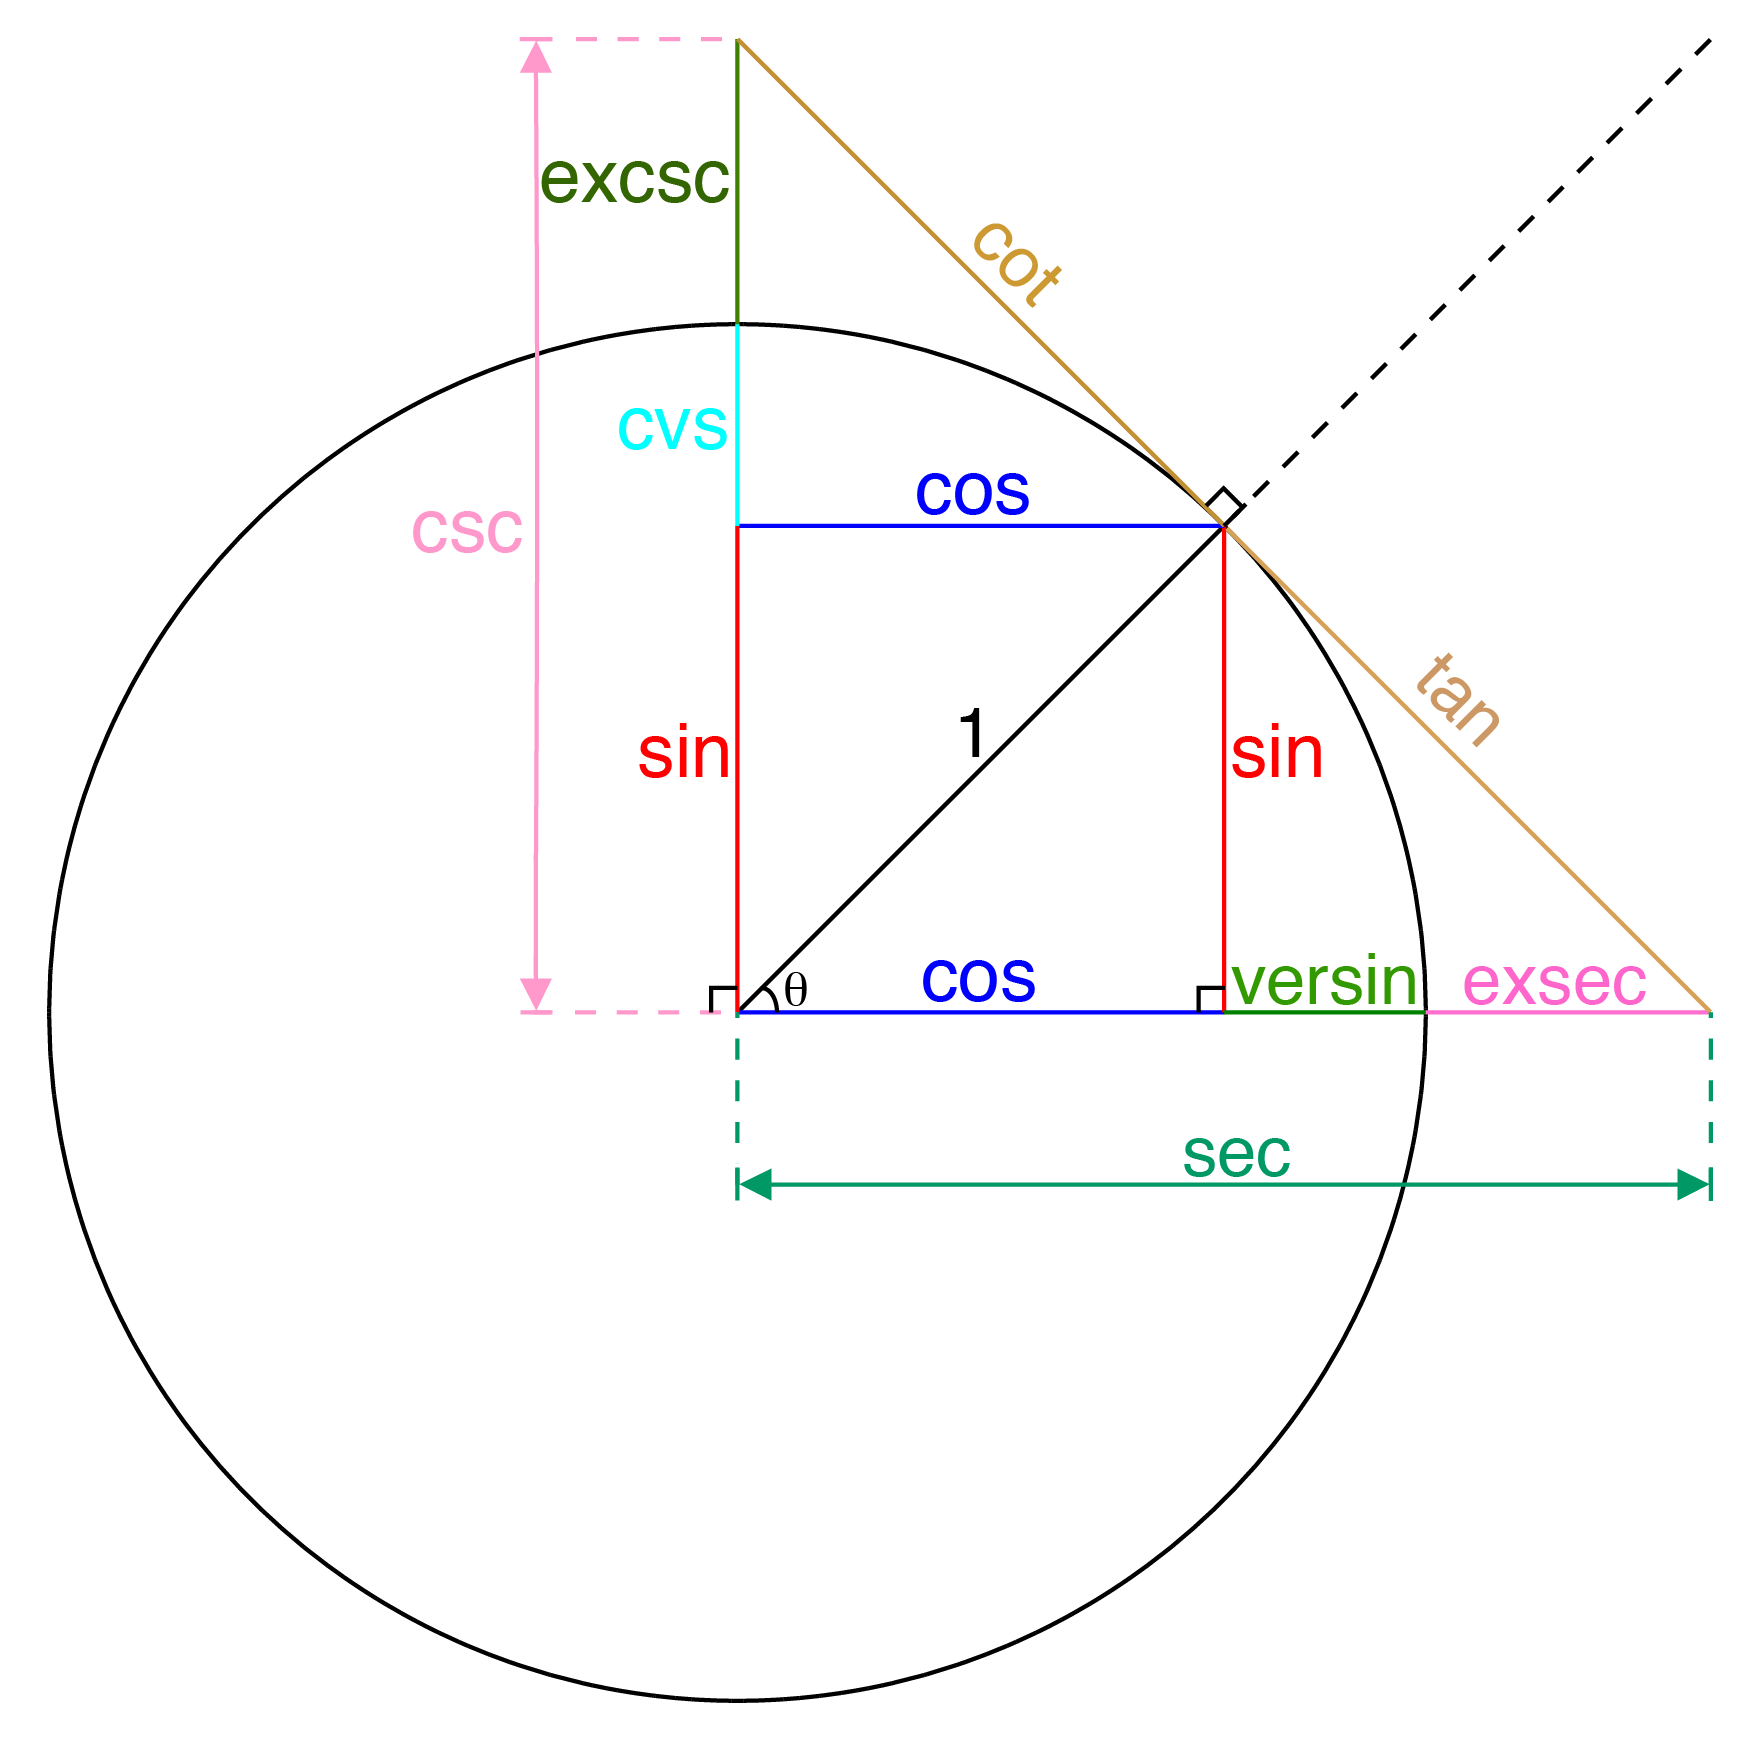
\includegraphics[width=\linewidth]{circle}
	%\captionof{figure}{my caption of the figure}
\end{Figure}
\subsection{Domain and Range}
\begin{itemize}[leftmargin=0.5em, label={·}]
	\item $\sin:\R\longrightarrow[-1,1]$
	\item $\cos:\R\longrightarrow[-1,1]$
	\item $\tan:\left\{x \in \R \ \middle| \ x \neq \frac{\pi}{2} + k\pi\right\}\longrightarrow\R$
	\item $\cot:\left\{x \in \R \ \middle| \ x \neq k\pi\right\}\longrightarrow\R$
	\item $\csc:\left\{x \in \R \ \middle| \ x \neq k\pi\right\}\longrightarrow\R \setminus \left(-1,1\right)$
	\item $\sec:\left\{x \in \R \ \middle| \ x \neq \frac{\pi}{2} + k\pi\right\}\longrightarrow\R \setminus \left(-1,1\right)$
	\item $\sin^{-1}: \left[-1,1\right] \longrightarrow \left[-\frac{\pi}{2},\frac{\pi}{2}\right]$
	\item $\cos^{-1}: \left[-1,1\right] \longrightarrow \left[0,\pi\right]$		
	\item $\tan^{-1}: \R \longrightarrow \left[-\frac{\pi}{2},\frac{\pi}{2}\right]$
\end{itemize}
\subsection{Pythagorean Identities}	
\begin{eqlist}
	\item $\sin^2(x) + \cos^2(x) = 1$
	\item $\tan^2(x) + 1 = \sec^2(x)$
	\item $1 + \cot^2(x) = \csc^2(x)$
\end{eqlist}

\subsection{Periodicity Identities}
\begin{eqlist}
	\item $\sin(x \pm 2\pi) = \sin(x)$
	\item $\cos(x \pm 2\pi) = \cos(x)$
	\item $\tan(x \pm \pi) = \tan(x)$
	\item $\cot(x \pm \pi) = \cot(x)$
	\item $\csc(x \pm 2\pi) = \csc(x)$
	\item $\sec(x \pm 2\pi) = \sec(x)$
\end{eqlist}

\subsection{Reciprocal Identities}	
\begin{eqlist}
	\item $\cot(x) = \frac{1}{\tan(x)}$
	\item $\csc(x) = \frac{1}{\sin(x)}$
	\item $\sec(x) = \frac{1}{\cos(x)}$
\end{eqlist}

\subsection{Quotient Identities}	
\begin{eqlist}
	\item $\tan(x) = \frac{\sin(x)}{\cos(x)}$
	\item $\cot(x) = \frac{\cos(x)}{\sin(x)}$
\end{eqlist}

\subsection{Sum Identities}	
\begin{eqlist}
	\item $\sin(x + y) = \sin(x)\cos(y) + \cos(x)\sin(y)$
	\item $\cos(x + y) = \cos(x)\cos(y) - \sin(x)\sin(y)$
	\item $\tan(x + y) = \frac{\tan(x) + \tan(y)}{1-\tan(x)\tan(y)}$
\end{eqlist}

\subsection{Difference Identities}	
\begin{eqlist}
	\item $\sin(x - y) = \sin(x)\cos(y) - \cos(x)\sin(y)$
	\item $\cos(x - y) = \cos(x)\cos(y) + \sin(x)\sin(y)$
	\item $\tan(x - y) = \frac{\tan(x) - \tan(y)}{1 + \tan(x)\tan(y)}$
\end{eqlist}

\subsection{Double Angle Identities}	
\begin{eqlist}
	\item $\sin(2x) = 2\sin(x)\cos(x)$
	\item $\cos(2x) = \cos^2(x) - \sin^2(x) $
	\item $\cos(2x) = 2\cos^2(x) - 1 \Rightarrow \cos^2(x) = \frac{\cos(2x)+1}{2}$
	\item $\cos(2x) = 1 - 2\sin^2(x) \Rightarrow \sin^2(x) = \frac{1-\cos(2x)}{2}$
	\item $\tan(2x) = \frac{2\tan(x)}{1-\tan^2(x)} $
\end{eqlist}

\subsection{Co-Function Identities}	
\begin{eqlist}
	\item $\sin\left(\frac{\pi}{2}-x\right) = \cos(x)$
	\item $\cos\left(\frac{\pi}{2}-x\right) = \sin(x)$
	\item $\tan\left(\frac{\pi}{2}-x\right) = \cot(x)$
	\item $\cot\left(\frac{\pi}{2}-x\right) = \tan(x)$
	\item $\csc\left(\frac{\pi}{2}-x\right) = \sec(x)$	
	\item $\sec\left(\frac{\pi}{2}-x\right) = \csc(x)$
\end{eqlist}

\subsection{Even-Odd Identities}	
\begin{eqlist}
	\item $\sin(-x) = -\sin(x)$
	\item $\cos(-x) = \cos(x)$
	\item $\tan(-x) = -\tan(x)$
	\item $\cot(-x) = -\cot(x)$
	\item $\csc(-x) = -\csc(x)$
	\item $\sec(-x) = \sec(x)$
\end{eqlist}

\subsection{Half-Angle Identities}	
\begin{eqlist}
	\item $\sin\left(\frac{x}{2}\right) = \pm\sqrt{\frac{1-\cos(x)}{2}}$
	\item $\cos\left(\frac{x}{2}\right) = \pm\sqrt{\frac{1+\cos(x)}{2}}$
	\item $\tan\left(\frac{x}{2}\right) = \pm\sqrt{\frac{1-\cos(x)}{2}}$
	\item $\tan\left(\frac{x}{2}\right) = \frac{1-\cos(x)}{\sin(x)}$
	\item $\tan\left(\frac{x}{2}\right) = \frac{\sin(x)}{1+\cos(x)}$
\end{eqlist}

\subsection{Sum-to-Product Formulas}
\begin{eqlist}
	\item $\sin(x) + \sin(y) = 2\sin\left(\frac{x+y}{2}\right)\cos\left(\frac{x-y}{2}\right)$
	\item $\sin(x) - \sin(y) = 2\sin\left(\frac{x-y}{2}\right)\cos\left(\frac{x+y}{2}\right)$
	\item $\cos(x) + \cos(y) = 2\cos\left(\frac{x+y}{2}\right)\cos\left(\frac{x-y}{2}\right)$
	\item $\cos(x) - \cos(y) = -2\sin\left(\frac{x+y}{2}\right)\cos\left(\frac{x-y}{2}\right)$
\end{eqlist}

\subsection{Product-to-Sum Formulas}
\begin{eqlist}
	\item $\sin(x)\sin(y) = \frac{1}{2}\left[\cos(x-y)-\cos(x+y)\right]$
	\item $\cos(x)\cos(y) = \frac{1}{2}\left[\cos(x-y)+\cos(x+y)\right]$
	\item $\sin(x)\cos(y) = \frac{1}{2}\left[\sin(x+y)+\sin(x-y)\right]$
	\item $\cos(x)\sin(y) = \frac{1}{2}\left[\sin(x+y)-\sin(x-y)\right]$
\end{eqlist}

\subsection{Tangent expression}
If $u = \tan(\frac{x}{2}):$ $\ \ \ \left[dx = \frac{2}{1+u^2}du\right]$
\begin{eqlist}
	\item $\cos(x) = \frac{1-u^2}{1+u^2}$
	\item $\sin(x) = \frac{2u}{1+u^2}$
	\item $\tan(x) = \frac{2u}{1-u^2}$
\end{eqlist}

\subsection{Hyperbolic Functions} 
\begin{eqlist}
	\item $\sinh(x) = \frac{e^x-e^{-x}}{2}$
	\item $\cosh(x) = \frac{e^x+e^{-x}}{2}$
	\item $\tanh(x) = \frac{e^x-e^{-x}}{e^x+e^{-x}}$
\end{eqlist}

\subsection{Laws of Sines}
\begin{eqlist}
	\item $\frac{\sin(\alpha)}{a} = \frac{\sin(\beta)}{b} = \frac{\sin(\gamma)}{c}$
\end{eqlist}

\subsection{Laws of Cosines}
\begin{eqlist}
	\item $a^2 = b^2 + c^2 - 2bc\cos(\alpha)$
	\item $b^2 = a^2 + c^2 - 2ac\cos(\beta)$
	\item $c^2 = a^2 + b^2 - 2ab\cos(\gamma)$
\end{eqlist}

\subsection{Degrees}
\begin{Figure}
	\centering
	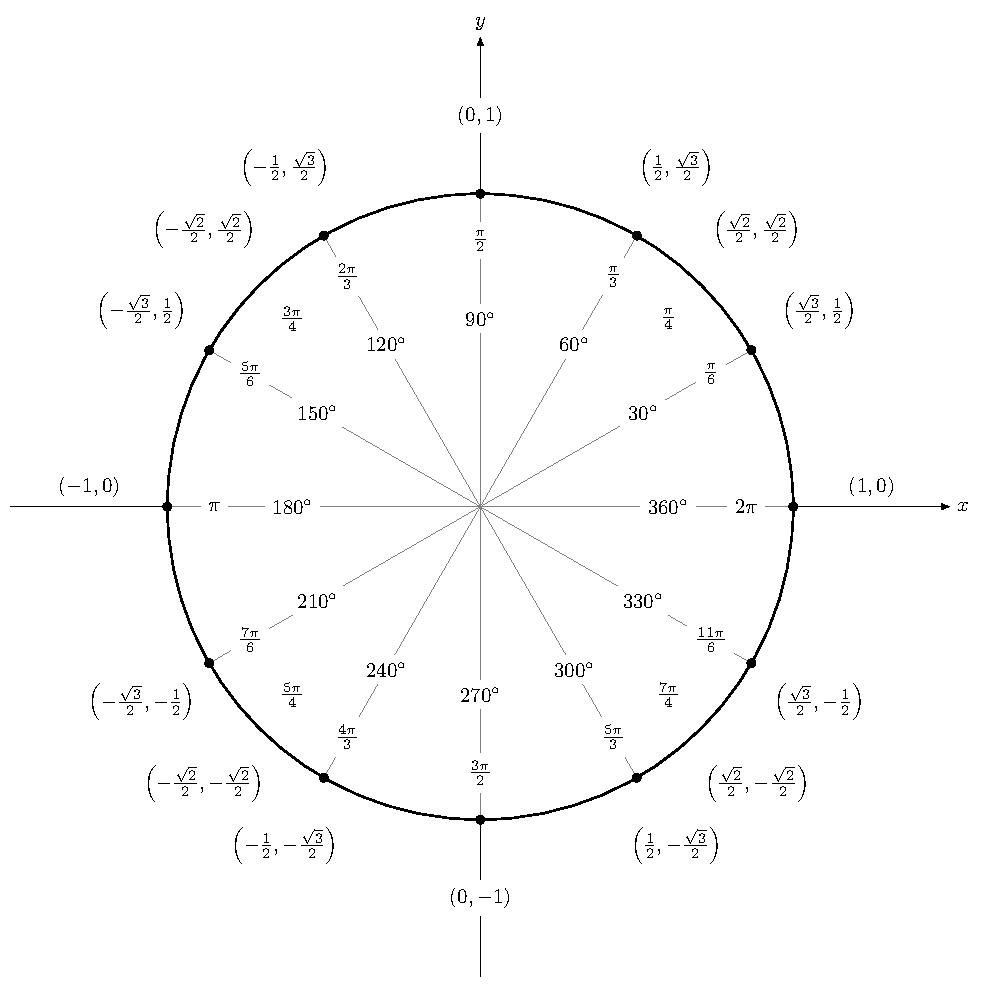
\includegraphics[width=\linewidth]{degrees_circle}
	%\captionof{figure}{my caption of the figure}
\end{Figure}

\begin{Figure}
	\centering
	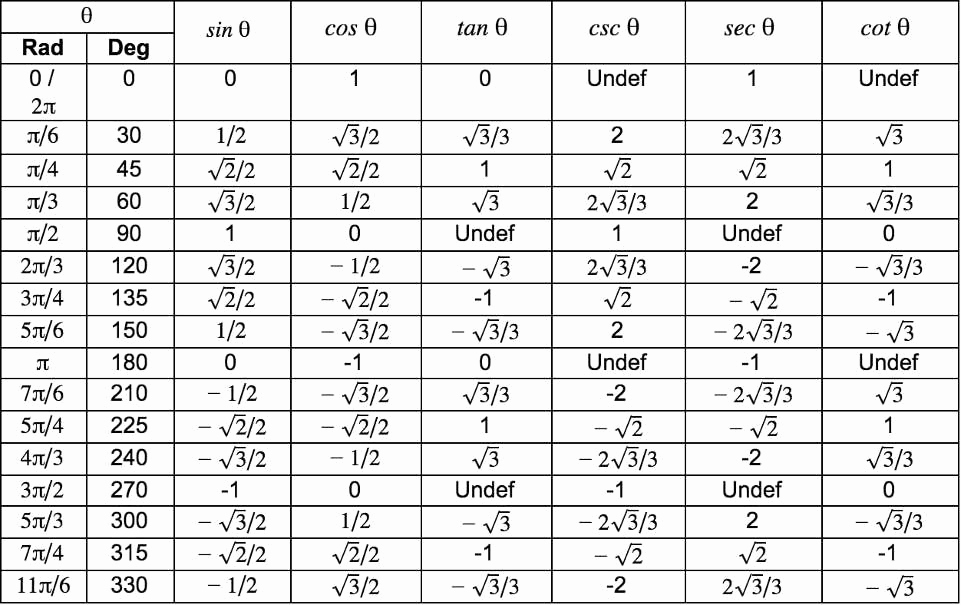
\includegraphics[width=\linewidth]{unit_circle_table}
\end{Figure}

\vfill\eject

\section{Limits, Sup and Inf}
\begin{boxdefinition}[Limits]
	Let $f(x)$ be a function defined on $D\subseteq \R$, let $x_0$ be a limit point in $D$, then we say that $\lim_{x\to x_0}f(x) = L\in\R$ if for all $\epsilon$ there exists a $\delta$ such that: 
	\[
		 \forall x \in D:\ 0 < |x-x_0| < \delta \Rightarrow |f(x) - L| < \epsilon
	\]
\end{boxdefinition}
\textbf{Sequence Definition:} \\ $\displaystyle\lim_{x\to x_0}f(x) = L \Leftrightarrow \forall (x_n)$ where $\displaystyle\lim_{n\to \infty}x_n = x_0$, then $\displaystyle\lim_{n\to \infty}f(x_n) = L$ 
\subsection{Limit Properties}
Assume that $\lim_{x \to x_0}f(x)$ and $\lim_{x \to x_0}g(x)$ exists and that $c\in\R$, then: 
\begin{eqlist}
	\item $\displaystyle\lim_{x \to x_0}[cf(x)] = c\lim_{x \to x_0}f(x)$
	\item $\displaystyle\lim_{x \to x_0}[f(x) \pm g(x)] = \lim_{x \to x_0}f(x) \pm \lim_{x \to x_0} g(x)$
	\item $\displaystyle\lim_{x \to x_0}[f(x)g(x)] = \lim_{x \to x_0}f(x) \lim_{x \to x_0}g(x)$
	\item $\displaystyle\lim_{x \to x_0}\left[\frac{f(x)}{g(x)}\right] = \frac{\displaystyle\lim_{x \to x_0}f(x)}{\displaystyle\lim_{x \to x_0}g(x)}, \lim_{x \to x_0}g(x) \neq 0$
	\item $\displaystyle\lim_{x \to x_0}[f(x)]^n = \left[\lim_{x \to x_0}f(x)\right]^n$
	\item $\displaystyle\lim_{x \to x_0}\left[\sqrt[n]{f(x)}\right] = \sqrt[n]{\lim_{x \to x_0}f(x)}$
	\item $\displaystyle\lim_{x \to x_0}x = x_0$
\end{eqlist}
\subsection{Chain Rule}
Let $f$ and $g$ be continuous, and given $\lim_{x \to x_0}f(g(x))$ of composed function we can solve $\lim_{x \to x_0}g(x) = y_0$, then: \\ 
$$\lim_{x \to x_0}f(g(x)) = \lim_{y \to y_0}f(y)$$
\subsection{Exponential Rule} 
Let $f$ and $g$ be continuous, where $\lim_{x\to x_0}f(x) = f(x_0) > 0$ and $\lim_{x\to x_0}g(x) = g(x_0)$ (where both limits exists), then:
$$\lim_{x \to x_0}f(x)^{g(x)} = f(x_0)^{g(x_0)}$$
\subsection{Root Trick}
$\displaystyle\lim_{x \to x_0} \sqrt{f}-g = \lim_{x \to x_0} \sqrt{f}- g \cdot \frac{\sqrt{f}+g}{\sqrt{f}+g}$
\subsection{E-Log Trick}
$\displaystyle\lim_{x \to x_0}f^g = \lim_{x \to x_0}e^{g\ln(f)}$
\begin{boxtheorem}[L'Hôpital's Rule ]
	If by plugging $x_0$ in $\frac{f(x)}{g(x)}$ we get $\frac{0}{0}$ or $\frac{\pm\infty}{\pm\infty}$, then: \\
	$$\displaystyle\lim_{x \to x_0}\frac{f(x)}{g(x)} = \lim_{x \to x_0}\frac{f'(x)}{g'(x)} = L \Leftrightarrow L \neq \pm\infty$$
\end{boxtheorem}
\begin{boxtheorem}[Limit Squeeze Theorem]
Let $\displaystyle\lim_{x \to x_0}f(x)$, if $g(x) \leq f(x) \leq h(x), \forall x$, and $\displaystyle\lim_{x \to x_0}g(x) = \lim_{x \to x_0}h(x) = L$, then: \\$$\displaystyle\lim_{x \to x_0}f(x) = L$$
\end{boxtheorem}
\subsection{Important Limits}
\begin{bulletlist}
	\item $\displaystyle\lim_{n \to \infty}\left(1 + \frac{x}{n}\right)^n = e^x$
	\item $\displaystyle\lim_{n \to 0} \frac{a^n-1}{n} = \ln(a)$
	\item $\displaystyle\lim_{n \to \infty} \ln(n) = \infty$
	\item $\displaystyle\lim_{n \to \infty} \frac{\log_{a}(1+n)}{n} = \frac{1}{\ln(a)}$			
	\item $\displaystyle\lim_{n \to 0} \frac{\log_{a}(1+n)}{n} = \frac{1}{\ln(a)}$
	\item $\displaystyle\lim_{n \to 0} \frac{\sin(n)}{n} = 1$
	\item $\displaystyle\lim_{n \to 0} \frac{1-\cos(n)}{n} = 0$
	\item $\displaystyle\lim_{n \to 0} \frac{1-\cos(n)}{n^2} = \frac{1}{2}$
	\item $\displaystyle\lim_{n \to 0} \frac{\tan(n)}{n} = 1$
	\item $\displaystyle\lim_{n \to \infty} \frac{n!}{n^n} = 0$
	\item $\displaystyle\lim_{n \to 0} \frac{e^n-1}{n} = 1$
	\item $\displaystyle\lim_{n \to \infty} \sqrt[n]{n!} = \infty$
	\item $\displaystyle\lim_{n \to \infty} \sqrt[n]{n} = 1$
\end{bulletlist}
\subsection{Strategy}
Given a limit $\displaystyle\lim_{x \to x_0}f(x)$:
\begin{numberlist}
	\item Is $f(x_0)$ solvable normally (polynomials and radicals) ?
	\item Try to decompose the limit with the properties and go back to step 1 for each piece.
	\item If it contains a \textbf{radical expession} try with the root trick, pay attention that if it's not a square root you can try with the third root factorization, but for bigger roots it's probabily another method. If the root contains the entire limit it can be put out (PR6).
	\item If it contains a \textbf{trigonometric function} try with the Squeeze Theorem, if the trig function contains another function go with the composed function decomposition. If it simplifies well with the series definition of $\cos,\sin,$ or $\tan$ try to simplify the sum and solve each piece.
	\item If it's a \textbf{composed function} try the chain rule.
	\item If it's raised to an \textbf{unusual power} try the E-Log trick. 
	\item If you get $\frac{0}{0}$ or $\frac{\pm\infty}{\pm\infty}$ use l'Hopital. 
	\item If you get $\pm\infty\cdot 0$ or $0\cdot\pm\infty$ tranform the function into a fraction so that you get $\frac{0}{0}$ or or $\frac{\pm\infty}{\pm\infty}$ then use l'Hopital. 

\end{numberlist}

\subsection{Supremum and Infimium}
\begin{boxdefinition} 
	\
	\begin{bulletlist}
		\item The \textbf{Supremum} of a set $S$ denoted $sup(S) = u$ is a number $u$ that satisfies the condition that $u$ is an upper bound of $S$ and for any upper bound $v$ of $S$, $u\leq v$.
		\item The \textbf{Infimium} of a set $S$ denoted $inf(S) = u$ is a number $u$ that satisfies the condition that $u$ is an lower bound of $S$ and for any lower bound $v$ of $S$, $u\geq v$.
	\end{bulletlist}
\end{boxdefinition}
\begin{bulletlist}
	\item If the supremum doesn't exists we can write:\\ $sup(S) = \infty$.
	\item If the infimium doesn't exist we can write:\\ $inf(S) = -\infty$.
	\item To prove that the minimum doesn't exist: \\ $\forall \epsilon \exists n_0 \in \N: f(x) \leq inf(a) + \epsilon \  \forall x \geq n_0$.
	\item To prove that the maximum doesn't exist: \\ $\forall \epsilon \exists n_0 \in \N: f(x) \leq sup(a) - \epsilon \  \forall x \geq n_0$.
\end{bulletlist}

\vfill\null
\columnbreak
\section{Continuity}
\begin{boxdefinition}[Pointwise Contiunous] \ \\ 
	A function $f:[a,b]\rightarrow\R$ is \textbf{pointwise continuous} at $x_0\in[a,b]$ if $\lim_{x\to x_0}f(x) = f(x_0)$, or:
	$$\forall \epsilon \exists \delta \ \forall x : (|x-x_0| < \delta \Rightarrow |f(x)-f(x_0)| < \epsilon)$$
\end{boxdefinition}
\begin{boxdefinition}[Uniformly Continuous] \ \\
	A function $f:[a,b]\rightarrow \R$ is \textbf{uniformly continuous} if it's continuous at every point in it's domain $\forall x_0 \in [a,b]: \lim_{x\to x_0}f(x) = f(x_0)$, or:
	$$\forall\epsilon\exists\delta \ \forall x_0, x: (|x-x_0| < \delta \Rightarrow |f(x)-f(x_0)| < \epsilon)$$
\end{boxdefinition}
\begin{boxdefinition}[Lipschitz Continuous] \ \\
	A function $f:[a,b]\rightarrow \R$ is \textbf{Lipschitz continuous} if:
	$$\exists L \forall x, x_0: |f(x)-f(x_0)| \leq L|x-x_0|$$ 
\end{boxdefinition}
\subsection{Properties}
Let $f$ and $g$ be continuous, then also $f\pm g$, $f \cdot g$, $\frac{f}{g} \Leftrightarrow g\neq 0$ and $f \circ g$ are continuous. 
\begin{eqlist}
	\item \textbf{Polynomials:} All polynomials $P(x)$ are pointwise continuous on any bounded interval.
	\item \textbf{Bijective: } If $f:[a,b]\rightarrow\R$ is continuous and monotone, then it's bijective and $f^{-1}$ is also continuous.
\end{eqlist}

\begin{boxtheorem}[Intermediate Value]
	Let $f$ be a continuous function on $[a,b]$ and let $s$ be a number with $f(a) < s < f(b)$, then there exists at least one solution to $f(x) = s$.
\end{boxtheorem}
\begin{boxtheorem}[Extreme Value]
	Let $f:I\rightarrow \R$ be a continuous function on $I=[a,b]$ then there exist two numbers $c \in I$ and $d \in I$ such that:
	$$\forall x \in I: \ m = f(c) \leq f(x) \leq f(d) = M$$
	Where $m$ is a lower bound and $M$ an upper bound.
\end{boxtheorem}

\vfill\eject
\columnbreak
\section{Derivatives}
\begin{boxdefinition}[Derivative]
	The \textbf{derivative} of $f(x)$ with respect to $x$ is: \\
	\[
	\begin{split}
		\displaystyle\frac{df}{dx} = f'(x) &= \lim_{h \to 0}\frac{f(x+h)-f(x)}{h}\\ 
		&=\lim_{x_0 \to x} \frac{f(x_0)-f(x)}{x_0-x}
	\end{split}
	\]
\end{boxdefinition}
\subsection{Properties}
\begin{eqlist}
	\item $\frac{d}{dx}(c) = 0$
	\item $(cf)' = cf'(x)$
	\item $(f\pm g)'= f'(x) + g'(x)$
	\item $(fg)' = f'g + fg'$
	\item $\left(\frac{f}{g}\right)' = \frac{f'g-fg'}{g^2}$
	\item $\frac{d}{dx}\left([f(x)]^n\right) = n[f(x)]^{n-1}f'(x)$
	\item $\frac{d}{dx}(f(g(x)) = f'(g(x))g'(x)$
	\item $[f^{-1}]'(x) = \frac{1}{f'(f^{-1}(x))}$
\end{eqlist}
\subsection{Common Derivatives}
\begin{bulletlist}
	\item $\frac{d}{dx}(x) = 1$
	\item $\frac{d}{dx}(|x|) = sign(x)$
	\item $\frac{d}{dx}(e^x) = e^x$	
	\item $\frac{d}{dx}(a^x) = a^x\ln(a)$
	\item $\frac{d}{dx}(\frac{1}{x}) = -\frac{1}{x^2}$
	\item $\frac{d}{dx}\sqrt{x} = \frac{1}{2\sqrt{x}}$
	\item $\frac{d}{dx}(\ln(f(x))) = \frac{f'(x)}{f(x)} = \frac{1}{x} \ \textit{if} \ f(x) = x$
	\item $\frac{d}{dx}(\ln|x|) = \frac{1}{x},\ x\neq0$
	\item $\frac{d}{dx}(\log_{a}(x)) = \frac{1}{xln(a)},\ x>0$
	\item $\frac{d}{dx}(\sin(x)) = \cos(x)$
	\item $\frac{d}{dx}(\cos(x)) = -\sin(x)$
	\item $\frac{d}{dx}(\tan(x)) = \sec^2(x) = \tan^2(x)+1$
	\item $\frac{d}{dx}(\cot(x)) = -\csc^2(x)$
	\item $\frac{d}{dx}(\sec(x)) = \sec(x)\tan(x)$
	\item $\frac{d}{dx}(\csc(x)) = -\csc(x)\cot(x)$
	\item $\frac{d}{dx}(\sin^{-1}(x)) = \frac{1}{\sqrt{1-x^2}}$
	\item $\frac{d}{dx}(\cos^{-1}(x)) = -\frac{1}{\sqrt{1-x^2}}$
	\item $\frac{d}{dx}(\tan^{-1}(x)) = \frac{1}{1+x^2}$
	\item $\frac{d}{dx}(\sinh(x)) = \cosh(x)$
	\item $\frac{d}{dx}(\cosh(x)) = \sinh(x)$
	\item $\frac{d}{dx}(\tanh(x)) = \frac{1}{\cosh(x)} = 1-\tanh^2(x)$
	\item $\frac{d}{dx}(\sinh^{-1}(x)) = \frac{1}{\sqrt{x^2+1}}$
	\item $\frac{d}{dx}(\cosh^{-1}(x)) = \frac{1}{\sqrt{x^2-1}}$
	\item $\frac{d}{dx}(\tanh^{-1}(x)) = \frac{1}{\sqrt{1-x^2}}$
\end{bulletlist}

\subsection{Differentiable}
\begin{boxtheorem}[Differentiable]
	A function $f$ is differentiable at a point $x_0$ iff:
	$$\lim_{x \to x_{0}^+} \frac{f(x)-f(x_0)}{x-x_0} = \lim_{x \to x_{0}^-} \frac{f(x)-f(x_0)}{x-x_0}$$
\end{boxtheorem}
\begin{eqlist}
	\item \textbf{Tangent Line:} The function $f$ has a tangent point at $a$ if and only if $f$ is differentiable at $a$. The equation of the tangent line is:
	$$y = f'(a)(x-a)+f(a)$$
	\item \textbf{Continuous:} If $f(x)$ is differentiable at $a$, then $f$ is continuous at $a$. The converse is not true (e.g. $f(x) = |x|, \ a=0$).
	\item \textbf{Classes:} If $f:[a,b] \rightarrow \R$ is differentiable $k$ times we say that $f \in C^k([a,b])$ where $C$ is called \textit{classification function}. If $f$ is differentiable infinite times we say that $f$ is \textit{smooth} ($f \in C^\infty([a,b])$). 
\end{eqlist}

\begin{boxtheorem}[Inverse Function Theorem]
	Let $f: [a,b] \longrightarrow \R$ be continuous, differentiable and stricly increasing where $\forall x\in[a,b]: f'(x)>0$ and $$c = \underset{a<x<b}{\inf} f(x) < \underset{a<x<b}{\sup} f(x) = d$$ then: 
	\begin{bulletlist}
		\item $f:\left]a,b\right[\rightarrow\left]c,d\right[$ is bijective.
		\item $f^{-1}:\left]c,d\right[\rightarrow\left]a,b\right[$ is differentiable with $[f^{-1}]'(x) = \frac{1}{f'(f^{-1}(x))}$
	\end{bulletlist}
\end{boxtheorem}

\begin{boxtheorem}[Mean Value Theorem]
	Let $f: [a,b] \longrightarrow \R$ be continuous and differentiable on $\left]a,b\right[$, then exists $c\in\left]a,b\right[$ with: \\
	$f(b) = f(a) + f'(c)(b-a) \text{, or:}$
	$$f'(c) = \frac{f(b)-f(a)}{b-a}$$
\end{boxtheorem}


\vfill\null
\columnbreak
\vfill\null
\columnbreak

\section{Integrals}
\begin{boxdefinition}[Riemann-Integral]
	Given:
	\begin{bulletlist}
		\item A continuous function $f(x): [a,b] \longrightarrow \R$
		\item A partition $P \defeq \{a=x_0,...,x_{n-1}, x_n=b\} $ where $I_i = [x_{i-1}, x_i]$
		\item A set of points $\xi \defeq \{\xi_1,...,\xi_n\}$ where \\$\xi_i\in I_i = [x_{i-1}, x_i]$.
	\end{bulletlist}
	Then the Riemann-Sum is defined as: 
	$$S(f, P, \xi) \defeq \sum_{i=1}^n f(\xi_i) \cdot (x_i-x_{i-1})$$
	Where the \textbf{Riemann-Integral} is: 
	$$\int_{a}^{b} f(x)dx \defeq \lim_{n\to\infty}\sum_{i=1}^n f(\xi_i) \cdot (x_i-x_{i-1})$$
\end{boxdefinition}
\begin{eqlist}
	\item \textbf{Over Sum:} \\
	$\displaystyle\overline{S}(f, P) \defeq \lim_{n\to\infty}\sum_{i=1}^n \underset{x\in I_i}{\sup}f(x) \cdot (x_i-x_{i-1})$\\
	\textbf{Infimum of the over sum:} \\
	$\displaystyle\underset{P}{\inf}\overline{S}(f, P) \defeq (b-a)\cdot\lim_{n\to\infty} \frac{1}{n} \sum_{i=1}^n \underset{x\in I_i}{\sup}f(x)$
	\item \textbf{Under Sum:} \\
	$\displaystyle\underline{S}(f, P) \defeq \lim_{n\to\infty}\sum_{i=1}^n \underset{x\in I_i}{\inf}f(x) \cdot (x_i-x_{i-1})$\\
	\textbf{Supremum of the under sum:} \\
	$\displaystyle\underset{P}{\sup}\underline{S}(f, P) \defeq (b-a)\cdot\lim_{n\to\infty} \frac{1}{n} \sum_{i=1}^n \underset{x\in I_i}{\inf}f(x)$
	\item[] $\displaystyle I_i = \left[a+\frac{(i-1)(b-a)}{n}, a+\frac{i(b-a)}{n}\right]$
	\item \textbf{Inequality:} \\
	$\underset{p\in P(I)}{\sup}\underline{S}(f, P) \leq \underset{p\in P(I)}{\inf}\overline{S}(f, P)$
	\item \textbf{Monotone:} A monotone function $f:I \rightarrow \R$ is Riemann-Integrable over $I$.
	\item \textbf{Continuous:} A continuous function $f:I \rightarrow \R$ is Riemann-Integrable over $I$.
\end{eqlist}
\begin{boxtheorem}[Riemann-Integrable] 
	A function $f$ is Riemann-Integrable iff: 
	$$\underset{P_1}{\sup}\underline{S}(f, P) = \underset{P_2}{\inf}\overline{S}(f, P)$$
	More formally: 
	$$\forall \epsilon \exists P: |\underline{S}(f, P) - \overline{S}(f, P)| < \epsilon$$

\end{boxtheorem}
\subsection{Properties}
\begin{eqlist}
	\item $\int_{a}^{a} f(x)dx = 0$
	\item $\int_{a}^{b} cf(x) = c\int_{a}^{b} f(x)$
	\item $\int_{a}^{b} f(x)+g(x)dx = \int_{a}^{b} f(x)dx \pm \int_{a}^{b} g(x)dx$
	\item $\int_{a}^{b} f(x)dx = -\int_{b}^{a}f(x) dx$
	\item $\int_{a}^{b} f(x)dx = \int_{a}^{c} f(x)dx + \int_{c}^{b} f(x)dx$
	\item $\int_{a}^{b} cdx = c(b-a)$
	\item If $f(x) \geq g(x)$, then: \\
	$\int_{a}^{b} f(x) \geq \int_{a}^{b} g(x)$
	\item If $m \leq f(x) \leq M$, then: \\
	$m(b-a) \leq \int_{a}^{b}f(x)dx \leq M(b-a)$
	\item If $\left|\int_{a}^{b}f(x)dx\right|\leq \int_{a}^{b}|f(x)|dx$
\end{eqlist}


\subsection{Common Integrals ($+C$)}
\begin{bulletlist}
	\item [] \textbf{Basic}
	\item $\int kdx = kx$
	\item $\int x^ndx = \frac{x^{n+1}}{n+1}, \ n\neq-1$
	\item $\int \frac{1}{x^n} = \frac{-1}{(n-1)x^{n-1}}$
	\item $\int x^{-1}dx = \int \frac{1}{x}dx = \ln|x|$
	\item $\int a^x dx = \frac{a^x}{ln(a)}$
	\item $\int e^x dx = e^x$
	\item $\int \log_a(x)dx = x\log_a(x)-x\log_a(e)$
	\item [] \textbf{Trigonometirc}
	\item $\int \sin(x)dx = -\cos(x)$
	\item $\int \cos(x)dx = \sin(x)$
	\item $\int \tan(x)dx = -\ln|\cos(x)| = \ln|\sec(x)|$
	\item $\int \cot(x)dx = \ln|\sin(x)|$
	\item $\int \sec(x)dx = \ln|\sec(x)+\tan(x)|$
	\item $\int \csc(x)dx = -\ln|\csc(x)+\cot(x)|$
	\item $\int \sin^{-1}(x)dx = x\sin^{-1}(x)+\sqrt{1-x^2}$
	\item $\int \cos^{-1}(x)dx = x\cos^{-1}(x)-\sqrt{1-x^2}$
	\item $\int \tan^{-1}(x)dx = x\tan^{-1}(x)-\sqrt{1}{2}\ln(1+x^2)$
	\item $\int \cot^{-1}(x)dx = x\cot^{-1}(x)+\sqrt{1}{2}\ln(1+x^2)$
	\item $\int \sin^2(x)dx = \frac{1}{2}(x-\sin(x)\cos(x)$
	\item $\int \cos^2(x)dx = \frac{1}{2}(x+\sin(x)\cos(x)$
	\item $\int \tan^2(x)dx = \tan(x)-x$
	\item $\int \cot^2(x)dx = -\cot(x)-x$
	\item $\int \sec^2(x)dx = \tan(x)$
	\item $\int \csc^2(x)dx = -\cot(x)$
	\item $\int \csc(x)\cot(x)dx = -\csc(x)$ 
	\item $\int \frac{1}{\sin(x)}dx = \ln\left|\frac{1-\cos(x)}{\sin(x)}\right|$
	\item $\int \frac{1}{\cos(x)}dx = \ln\left|\frac{1+\sin(x)}{\cos(x)}\right|$
	\item $\int \frac{1}{\sin^2(x)}dx = -\cot(x)$
	\item $\int \frac{1}{\cos^2(x)}dx = \tan(x)$
	\item $\int \frac{1}{1+\sin(x)}dx = \frac{-\cos(x)}{1+\sin(x)}$
	\item $\int \frac{1}{1+\cos(x)}dx = \frac{\sin(x)}{1+\cos(x)}$
	\item $\int \frac{1}{1-\sin(x)}dx = \frac{\cos(x)}{1-\sin(x)}$
	\item $\int \frac{1}{1-\cos(x)}dx = \frac{-\sin(x)}{1-\cos(x)}$
	\item $\int \sin(ax)dx = -\frac{1}{a}\cos(ax)$
	\item $\int \cos(ax)dx = \frac{1}{a}\sin(ax)$
	\item $\int \tan(ax)dx = -\frac{1}{a}\ln(\cos(ax))$
	\item $\int x\sin(ax)dx = -\frac{1}{a}x\cos(ax)+\frac{1}{a^2}\sin(ax)$
	\item $\int x\cos(ax)dx = \frac{1}{a}x\sin(ax)+\frac{1}{a^2}\cos(ax)$
	\item $\int \sinh(x) dx = \cosh(x)$
	\item $\int \cosh(x) dx = \sinh(x)$
	\item $\int \tanh(x) dx = \ln(\cosh(x))$
	\item $\int \coth(x) dx = \ln|\sinh(x)|$
	\item $\int \sinh^{-1}(x) dx = x\sinh^{-1}(x) - \sqrt{x^2+1}$
	\item $\int \cosh^{-1}(x) dx = x\cosh^{-1}(x) - \sqrt{x^2-1}$
	\item $\int \tanh^{-1}(x) dx = x\tanh^{-1}(x) + \frac{1}{2}\ln(1-x^2)$
	\item $\int \coth^{-1}(x) dx = x\coth^{-1}(x) + \frac{1}{2}\ln(x^2-1)$
	\item [] \textbf{Logarithmic}
	\item $\int \ln(ax)dx = x\ln(ax)-x$
	\item $\int x\ln(ax)dx = \frac{x^2}{4}(2\ln(ax)-1)$
	\item $\int \frac{\ln(ax)}{x}dx = \frac{1}{2}(\ln(ax)^2$
	\item [] \textbf{Exponential}
	\item $\int e^{ax}dx = \frac{1}{a}e^{ax}$
	\item $\int xe^x dx = (x-1)e^x$
	\item $\int xe^{ax}dx = \left(\frac{x}{a}-\frac{1}{a^2}\right)e^{ax}$
	\item [] \textbf{Rational Functions}
	\item $\int \frac{1}{\sqrt{x}} = 2\sqrt{x}$
	\item $\int (x+a)^n dx=\frac{(x+a)^{n+1}}{n+1}, \ n\neq-1$
	\item $\int x(x+a)^n dx=\frac{(x+a)^{n+1}((n+1)x-a)}{(n+1)(n+2)}$	
	\item $\int \frac{ax+b}{cx+d}dx = \frac{ax}{c}-\frac{ad-bc}{c^2}\ln|cx+d|$
	\item $\int \frac{1}{(x+a)^2}dx = -\frac{1}{x+a}$
	\item $\int \frac{1}{ax+b}dx = \frac{1}{a}\ln|ax+b|$ 
	\item $\int \frac{1}{a^2+x^2}dx = \frac{1}{a}\tan^{-1}\left(\frac{x}{a}\right)$
	\item $\int \frac{1}{ax^2+bx+c}dx = \frac{2}{\sqrt{4ac-b^2}}\tan^{-1}\left(\frac{2ax+b}{\sqrt{4ac-b^2}}\right)$
	\item $\int \frac{1}{(x-a)(x-b)}dx = \frac{1}{a-b}\ln\left|\frac{x-a}{x-b}\right|$
	\item $\int \frac{x}{a^2+x^2}dx = \frac{1}{2}\ln\left|a^2+x^2\right|$
	\item $\int \frac{x^2}{a^2+x^2}dx = x-a\tan^{-1}\left(\frac{x}{a}\right)$
	\item $\int \frac{x^3}{a^2+x^2}dx = \frac{1}{2}x^2-\frac{1}{2}a^2\ln\left|a^2+x^2\right|$
	\item $\int \frac{x}{(x+a)^2}dx = \frac{a}{a+x}+ \ln\left|a+x\right|$
	\item $\int \frac{x}{ax^2+bx+c} = \frac{1}{2a}\ln\left|ax^2+bx+c\right|-\frac{b}{a\sqrt{4ac-b^2}}\tan^{-1}\left(\frac{2ax+b}{\sqrt{4ac-b^2}}\right)$
	\item [] \textbf{Square Roots}
	\item $\int \sqrt{x-a}dx = \frac{2}{3}(x-a)^{\frac{3}{2}}$
	\item $\int \sqrt{ax+b}dx = \left(\frac{2b}{3a}+\frac{2x}{3}\right)\sqrt{ax+b}$
	\item $\int \sqrt{x^2+a}dx = \frac{1}{2}x\sqrt{x^2+a}+\frac{a}{2}\ln|x+\sqrt{x^2+a}|$
	\item $\int \sqrt{a^2-x^2}dx = \frac{1}{2}x\sqrt{a^2-x^2}+\frac{a^2}{2}\sin^{-1}\left(\frac{x}{a}\right)$
	\item $\int x\sqrt{x-a}dx = \frac{2}{3}a(x-a)^{\frac{3}{2}}+\frac{2}{5}(x-a)^{\frac{5}{2}}$
	\item $\int x\sqrt{x^2 \pm a^2}dx = \frac{1}{3}(x^2 \pm a^2)^{\frac{3}{2}}$	
	\item $\int (ax+b)^{\frac{3}{2}}dx = \frac{2}{5a}(ax+b)^{\frac{5}{2}}$
	\item $\int \frac{1}{\sqrt{x^2 \pm a^2}}dx = \ln\left|x+\sqrt{x^2 \pm a^2}\right|$
	\item $\int \frac{1}{\sqrt{a^2-x^2}}dx = \sin^{-1}\left(\frac{x}{a}\right)$
	\item $\int \frac{1}{\sqrt{x\pm a}}dx = 2\sqrt{x\pm a}$
	\item $\int \frac{x}{\sqrt{x^2 \pm a^2}}dx = \sqrt{x^2 \pm a^2}$
	\item [] \textbf{Other}
	\item $\int x\sin(ax)dx = -\frac{1}{a}x\cos(ax)+\frac{1}{a^2}\sin(ax)$
	\item $\int x\cos(ax)dx = \frac{1}{a}x\sin(ax)+\frac{1}{a^2}\cos(ax) $
	\item $\int e^{bx} \sin(ax)dx = \frac{1}{a^2+b^2}e^{bx}\left(b\sin(ax)-a\cos(ax)\right)$
	\item $\int e^{bx} \cos(ax)dx = \frac{1}{a^2+b^2}e^{bx}\left(a\sin(ax)+b\cos(ax)\right)$
\end{bulletlist}

\vfill\null
\columnbreak

\subsection{U-Substitution}
The substitution, $u=g(x)$, $du=g'(x)dx$ is: \\
$\displaystyle\int_a^b f(g(x))g'(x)dx = \int_{g(a)}^{g(b)}f(u)du $
\subsection{Integration By Parts}
$\displaystyle\int_a^b f(x)g'(x)dx = \left[f(x)g(x)\right]_{a}^{b} - \int_a^b f'(x)g(x)dx$ 
\begin{bulletlist}
	\item $u=f(x), \qquad\quad v=g(x)$ 
	\item $du=f'(x)dx, \quad dv=g'(x)dx$
\end{bulletlist}
$[\int u dv = uv-\int v du]$. As a rule of thumb use the following order, $u$ should be the function that comes first beween: Logarthmic $\leftrightarrow$ Inverse trig. $\rightarrow$ Algebraic ($Ax^n$)  $\rightarrow$ Trigonimetric $\rightarrow$ Exponential ($k^x$).
\subsection{Trig-Function Trick}
For $\int \sin^n(x)\cos^m(x)dx$ evaluate the following: 
\begin{eqlist}
	\item \textbf{Deg(n) odd: } strip one $\sin$ out and convert the rest to $\cos$ with $\sin^2(x) = 1-\cos^2(x)$, then use substitution on $u=\cos(x)$.
	\item \textbf{Deg(m) odd: } strip one $\cos$ out and convert the rest to $\sin$ with $\cos^2(x) = 1-\sin^2(x)$, then use substitution on $u=\sin(x)$.
	\item \textbf{Deg(n) and Deg(m) both odd:} use either (i) or (ii).
	\item \textbf{Deg(n) and Deg(m) both even:} use double angle and/or half angle trig identities to reduce the integral. 
\end{eqlist}
For $\int \tan^n(x)\sec^m(x)dx$ evaluate the following:
\begin{eqlist}
	\item \textbf{Deg(n) odd: } strip one $\tan$ and one $\sec$ out, and convert the rest to $\sec$ using $\tan^2(x) = \sec^2(x)-1$, then use substitution on $u=\sec(x)$.
	\item \textbf{Deg(m) even: } strip 2 $\sec$ out and convert the rest to $\tan$ with $\sec^2(x) = 1+\tan^2(x)$, then use substitution on $u=\tan(x)$.
	\item \textbf{Deg(n) odd and Deg(m) even:} use either (i) or (ii).
	\item \textbf{Deg(n) even and Deg(m) odd:} Deal with each integral differently. 
\end{eqlist}
\subsection{Root-Trig Substitution Trick}
If the integrals is one of the following roots use the given substitution and formula to convert it to an integral involving trig functions. 
\begin{eqlist}
	\item $\sqrt{a^2-b^2x^2} \Longrightarrow x = \frac{a}{b}\sin(u)$, with property $\cos^2(x)=1-\sin^2(x)$.
	\item $\sqrt{b^2x^2-a^2} \Longrightarrow x = \frac{a}{b}\sec(u)$, with property $\tan^2(x)=1-\sec^2(x)$.
	\item $\sqrt{a^2+b^2x^2} \Longrightarrow x = \frac{a}{b}\tan(u)$, with property $\sec^2(x)=1+\tan^2(x)$.
\end{eqlist}
\subsection{Rational Functions}
Given an integral $\int \frac{P(x)}{Q(x)}dx$:
\begin{bulletlist}
	\item For $deg(P(x)) \geq deg(Q(x))$, then apply a polynomial division so that we get an equivalent integral $\int A(x) + \frac{R(x)}{Q(x)}dx$ where $\int \frac{R(x)}{Q(x)}dx$ is easier to solve. 
	\item For $deg(P(x)) < deg(Q(x))$, then factor $Q(x)$ as completely as possible and find the partial fraction decomposition (P.F.D) of the rational expression.  	
	\begin{numberlist}
		\item $Q(x) = (ax+b)(cx^2+dx+e)$, then the P.F.D. is:\\ $\frac{A}{ax+b} + \frac{B}{cx^2+dx+e}$
		\item $Q(x) = (ax+b)^n $, then the P.F.D. is:\\ $ \frac{A_1}{ax+b}+\frac{A_2}{(ax+b)^2}+ \cdots + \frac{A_n}{(ax+b)^n}$
	\end{numberlist}
\end{bulletlist} 

\subsection{Improper Integrals}
\textbf{Convergent,} if $\lim = k$ with $k$ finite. \\ 
\textbf{Divergent,} if $\lim = \pm\infty \lor D.N.E.$ \\ \\ 
\textbf{Infinite Limit:}
\begin{eqlist}
	\item $\int_a^\infty f(x)dx = \lim_{t\to\infty}\int_a^t f(x)dx$
	\item $\int_{-\infty}^{b} f(x)dx = \lim_{t\to-\infty}\int_{t}^{b} f(x)dx$
	\item $\int_{-\infty}^{\infty} f(x)dx = \int_{-\infty}^{c} f(x)dx+\int_c^\infty f(x)dx$ \\ provided that both integrals are convergent.
\end{eqlist}
\textbf{Discontinuous Integrand:}
\begin{eqlist}
	\item Discontinuity at $a$: \\ $\int_a^b f(x)dx = \lim_{t\to a^+}\int_t^b f(x)dx$
	\item Discontinuity at $b$: \\ $\int_a^b f(x)dx = \lim_{t\to b^-}\int_a^t f(x)dx$
	\item Discontinuity at $a$ and $b$ ($a<c<b$): \\ $\int_a^c f(x)dx + \int_c^b f(x)dx$, if both convergent. 
\end{eqlist}
\textbf{Convergence Tests:}
\begin{bulletlist}
	\item \textbf{Comparison Test:} If $f(x) \geq g(x) \geq 0$ on $\left[a,\infty\right[$, then: \\ 
	If $\int_a^\infty f(x)dx$ converges $\Rightarrow \int_a^\infty g(x)dx$ converges. \\ 
	If $\int_a^\infty g(x)dx$ diverges $\Rightarrow \int_a^\infty f(x)dx$ diverges. \\ 
	Useful: If $a>0 \Rightarrow \int_a^\infty \frac{1}{x^p}dx$ converges if $p>1$ and diverges if $p\leq1$.
	\item \textbf{Limit Comparison Test:} If $f,g$ are continuous on $\left[a,\infty\right[$ with $\lim_{x\to\infty} \frac{f(x)}{g(x)}=L\neq\infty$, then: \\
	$\int_a^\infty |f(x)|dx$ converges $\Leftrightarrow \int_a^\infty |g(x)|dx$ converges
	\item \textbf{Absolute Converpgence:} \\ $\int_a^\infty |f(x)|dx$ converges $\Rightarrow \int_a^\infty f(x)$ converges
\end{bulletlist}
\begin{boxdefinition}[Antiderivative] \ \\ 
	Let $f:[a,b]\rightarrow\R$ be a function where $$f(x) = F'(x) \ \forall x\in[a,b]$$ then $F$ is called the \textbf{antiderivative} of $f$.
\end{boxdefinition}	
\begin{boxtheorem}[Mean Value Theorem]
	\textit{(Integration)} Let $f$ be continuous on $[a,b]$, then there exists a $c$ such that: $$f(c) = \frac{1}{b-a}\int_a^b f(x)dx$$
	$(f(c) = f_{avg})$	
\end{boxtheorem}
\begin{boxtheorem}[Fundamental Theorem]
	\textbf{Part 1}: Suppose that $f$ is continuous on $[a,b]$ and $F$ is defined as: $F(x) \defeq \int_a^x f(t)dt$, then F is differentiable on $\left]a,b\right[$ and for all $x\in\left]a,b\right[$: $$F'(x) = f(x) $$
	\textbf{Part 2:} Suppose that $f$ is continuous on $[a,b]$ and $F$ is the antiderivative of $f$, then: 
	$$\int_a^b f(x)dx = F(b) - F(a)$$  
\end{boxtheorem}
\subsection{Derivative of Integrals}
If we have to evaluate the derivative of an integral where $F(x) = \int_{a}^{g(x)}f(t)dt$, then by the first part of the Fundamental Theorem of Calculus (and the Chain Rule) we have: $F'(x) = f(g(x))\cdot g'(x)$. \\
If $F(x) = \int_{h(x)}^{g(x)}f(t)dt = \int_{a}^{g(x)}f(t)dt - \int_{a}^{h(x)}f(t)dt$, then $F'(x) = f(g(x))g'(x) - f(h(x))h'(x)$.

\vfill\eject
\columnbreak

\section{Sequences}
\begin{boxdefinition}[Sequence]
	A sequence is set of numbers in a specific order, more formally:
	$(a_n)_{n=1}^\infty$ is a function $f:\N \rightarrow \R$ where $f(n) = a_n$.  
\end{boxdefinition}
\begin{boxdefinition}[Convergence] \ \\
	A sequence $(a_n)$ is \textbf{convergent} to a value $L$ if $\lim_{n\to\infty}a_n = L$, or: \\
	$$\forall\epsilon>0\exists N\in\N \forall n\in\N: (n>N \Rightarrow |a_n-L|<\epsilon)$$
	If the limit doesn't exist ($\pm\infty$ or doesn't converge) we say that $(a_n)$ is \textbf{divergent}.
\end{boxdefinition}	
\textit{Inutition}: If for any small number $\epsilon$ there is, we can find a number $N(\epsilon)$ and $L$ such that all points of $a_n$ after $N$ are at most at distance $\epsilon$ from $L$, the series converges.  
\subsection{Convergence Criteria}
\begin{eqlist}
	\item \textbf{Linearity:} If $(a_n)$ converges to $a$, $(b_n)$ converges to $b$ and $k\in\N$, then $(ka_n+b_n)$ converges to $ka+b$. 
	\item \textbf{Multiplication:} If $(a_n)$ converges to $a$ and $(b_n)$ converges to $b$ then $(a_n\cdot b_n)$ converges to $a\cdot b$. 
	\item \textbf{Division:} If $(a_n)$ converges to $a$ and $(b_n)$ converges to $b\neq0$ then $(\frac{a_n}{b_n})$ converges to $\frac{a}{b}$. 
	\item \textbf{Uniqueness:} If $(a_n)$ is convergent to $a$, then: $\lim_{n\to\infty}a_n = a$ is unique. 
	\item \textbf{Subsequence:} If $(a_n)$ converges to $a$, then: any subsequence $(a_{nk})$ is also convergent to $a$.
	\item \textbf{Squeeze Theorem: }If we have 3 convergent sequences $\lim_{n\to\infty}a_n=\lim_{n\to\infty}c_n=L$, and $\lim_{n\to\infty}b_n=b$ where $a_n\leq b_n \leq c_n$, then $b=L$.
	\item \textbf{Absolute:} If $(a_n)$ is convergent to $a$, then: $|a_n|$ also converges and $\lim_{n\to\infty}|a_n|=|a|$.
	\item \textbf{Ratio Test:} Let $(a_n)$ be a sequence where $\forall n\in\N: a_n>0$, then if $\lim_{n\to\infty}\left|\frac{a_{n+1}}{a_n}\right| = a$ and $a<1$, $\lim_{n\to\infty}a_n = 0$.
	\item \textbf{Boundedness:} If $(a_n)$ converges, then $(a_n)$ is bounded. 
	\item \textbf{Monotone Convergence:} $(a_n)$ is monotone then it's convergent $\Leftrightarrow (a_n)$ is bounded. \\
	If $(a_n)$ is increasing and bounded $\Rightarrow \lim_{n\to\infty}a_n= sup\{a_n: n\in\N\}$ \\
	If $(a_n)$ is decreasing and bounded $\Rightarrow \lim_{n\to\infty}a_n= inf\{a_n: n\in\N\}$ 
\end{eqlist}
\subsection{Divergence Criteria}
\begin{eqlist}
	\item $(a_n)$ is divergent if it has two subsequence that converge to different limits.
	\item $(a_n)$ is divergent if it has a divergent subsequence. 
	\item $(a_n)$ is divergent if it's unbounded. 
\end{eqlist}

\subsection{Monotonicity}
\begin{boxdefinition} \ 
	\begin{bulletlist}		
		\item A sequence is \textbf{increasing} if: \\
		$\forall n:\ a_n < a_{n+1}$
		\item A sequence is \textbf{decreasing} if: \\
		$\forall n:\ a_n > a_{n+1}$
		\item A sequence is \textbf{monotonic} if it's either increasing or decreasing. 
	\end{bulletlist}
\end{boxdefinition}
\textbf{Lemma: } Every sequence has a monotonic subsequence.

\subsection{Boundedness}
\begin{boxdefinition} \ 
	\begin{bulletlist}		
		\item A sequence is \textbf{bounded above} if: \\ 
		$\exists M>0\forall n\in\N:\ a_n \leq M$ 
		\item A sequence is \textbf{bounded below} if: \\ 
		$\exists m>0\forall n\in\N:\ m \leq a_n$
		\item A sequence is \textbf{bounded} if it's either bounded above or below. 
	\end{bulletlist}
\end{boxdefinition}

\subsection{Cauchy Sequence}
\begin{boxdefinition}\ \\
	A sequence $(a_n)$ is \textbf{Cauchy} if: 
	$$\forall\epsilon >0\exists N\in\N: \forall m,n\geq N \Rightarrow |a_n-a_m| < \epsilon $$
\end{boxdefinition}
\textit{Inutition}: If for any small number $\epsilon$ there is, we can find a number $N$ such that all points of $a_n$ after $N$ are at most at distance $\epsilon$ from each other, the series is Cauchy. 
\begin{eqlist}
	\item \textbf{Cauchy Convergence Criterion:} \\ $(a_n)$ is convergent $\Leftrightarrow$ it's Cauchy. 
	\item \textbf{Cauchy Bounded:} If $(a_n)$ is cauchy, then it's also bounded. 
	\item \textbf{Linearity:} If $(a_n)$ is Cauchy, $(b_n)$ is Cauchy and $k\in\N$, then $(ka_n+b_n)$ is also Cauchy. 
\end{eqlist}
The advantage is that we don't have to find a limit $L$ to prove that the sequence converges. 

\subsection{Accumulation Points}
\begin{boxdefinition}\ \\
	A number $a$ is an \textbf{accumulation point} of $(a_n)$ if there exists a subsequence $(a_{n_k})$ that converges to a, or:
	$$\forall\epsilon > 0 \exists K \in \N: (k\geq K \Rightarrow |a_{n_k} - a| < \epsilon)$$
\end{boxdefinition}
\begin{eqlist}
	\item \textbf{Convergence:} If $(a_n)$ converges to $L$, then $L$ is the only accumulation point of $(a_n)$.
	\item \textbf{Boundedness}: If $(a_n)$ is bounded, then it has at least one accumulation point. 
	\item \textbf{Divercence:} If $a_n$ diverges, then it has no accumulation point. 
\end{eqlist}


\subsection{Strategy}
\begin{bulletlist}
	\item \textbf{Convergence:} Treat $(a_n)$ like a function and calculate the limit, if it exists it's convergent. If it's a recursive sequence use the Monotone Convergence Criteria by first proving that it's both monotonic increasing/decreasing and then that it's bounded above if increasing and bounded below if decreasing. To find the limit let $\lim_{n\to\infty}a_n = \lim_{n\to\infty}a_{n+1} = L$ and solve $L = a_\infty$ by plugging L inside of $a_n$.
	\item \textbf{Monotonicity:} To prove that the sequence is monotonic pick a candidate between increasing/decreasing and solve the inequality with $a_n, a_{n+1}$ to prove your candidate. If the sequence is recursive prove your candidate by induction. 
	\item \textbf{Boundedness:} Try to change $n$ in $a_n$ to make the sequence as small as possible to find a lower bound m, and similarly as big as possible to find an upper bound M. Give the result in terms of \\$m \leq a_n \leq M$.  
	If it's a recursive sequence pick a candidate of upper/lower bound and prove it by induction. 
\end{bulletlist}

\vfill\null 
\columnbreak
\section{Sequences of Functions}
\begin{boxdefinition}
	A \textbf{sequence of a function} $(f_n)$ is a list of functions $(f_1,f_2,...)$ such that each $f_n$ maps a given subset of $\R$ into $\R$:
	$$(f_n)_{n\in\N},\ f_n:I\subseteq\R\longrightarrow\R$$
\end{boxdefinition}
\subsection{Convergence}
\begin{boxdefinition}
	A sequence of a function $(f_n)$ can converge to a function $f(x)$ in two different ways: 
	\begin{bulletlist}
		\item \textbf{Pointwise} if $\forall x\in I $: 
		$$\lim_{n\to\infty} f_n(x)=f(x)$$
		\item \textbf{Uniformly} if $\forall x\in I $: 
		$$\lim_{n\to\infty}\sup_{x\in I} |f_n(x)-f(x)| = 0,\ \textit{or:}$$ 
		$$\forall \epsilon > 0 \ \exists N\in\N:\ n\geq N \Rightarrow |f_n(x)-f(x)| < \epsilon $$
	\end{bulletlist}
\end{boxdefinition}
\begin{eqlist}
	\item \textbf{Convergence:} If $(f_n)$ converges uniformly, then it also converges pointwise.
	\item \textbf{Continuity:} If $(f_n)$ converges uniformly, then $f$ is continuous.
	\item \textbf{Differentiability:} If $(f_n)$ converges pointwise to $f$, and $f_n'$ converges uniformly to the function $g$ on $\left]a,b\right[$, then $f$ is differentiable on $\left]a,b\right[$ and $f'=g$, or: 	$\lim_{n\to\infty}f_n'=\left(\lim_{n\to\infty}f_n\right)'=f'$
	\item \textbf{Integrability:} If a sequence of integrable function $f_n$ converges uniformly to $f$ on $[a,b]$, then $f$ is integrable and: \\
	$\lim_{n\to\infty}\int_a^b f_n(x)dx = \int_a^b \lim_{n\to\infty}\left(f_n(x)\right)dx = \int_a^b f(x)dx$
\end{eqlist}
\vfill\eject
\columnbreak

\section{Series}
\begin{boxdefinition}\
	\begin{bulletlist}
		\item A \textbf{partial sum} is the sum of the first $n$ numbers of $(a_n)_{n=1}^\infty$, or: 
		$s_n \defeq \sum_{i=1}^n a_i$
		\item An \textbf{infinite series} is the sum of all terms of an infinite sequence $(a_n)_{n=1}^\infty$, or: 
		$$\lim_{n\to\infty}s_n = \sum_{i=1}^\infty a_i \defeq \lim_{N\to\infty}\sum_{i=1}^N a_i$$
	\end{bulletlist}
\end{boxdefinition}
\subsection{Convergence}
\begin{boxdefinition}[Convergence] \ \\ 
	An infinite series is called \textbf{convergent} if: 
	\[
	\begin{split}
		\sum_{k=1}^\infty a_k \ \text{converges} &\Leftrightarrow \lim_{n\to\infty}\sum_{k=1}^n a_k \ \textit{exists}\\
		&\Leftrightarrow (s_n) \ \textit{converges}
	\end{split}
	\]
\end{boxdefinition}
\begin{eqlist}
	\item \textbf{Linearity: } 
	If $\sum_{i=0}^\infty a_i=a$, $\sum_{i=0}^\infty b_i = b$, and $c\in\R$, then: $\sum_{i=0}^\infty (c a_i+b_i) = ca+b$
	\item \textbf{Comparison:} If $\sum_{i=0}^\infty a_i=a$, $\sum_{i=0}^\infty b_i = b$, and $\forall n\in\N \ a_n\leq b_n $, then $a\leq b$.
	\item \textbf{Start Convergence:} $\sum_{i=0}^\infty a_i$ is convergent $\Leftrightarrow \sum_{i=N}^\infty a_i \ \forall N\in\N$ is convergent. 
	\item \textbf{Bounded Convergence:} If $(a_n)$ is ultimately positive and $(s_n)$ is abounded above, then $\sum_{i=0}^\infty a_i$ converges. Otherwise the series diverges to infinity. 
	\item \textbf{Unbounded Divergence:} If $(a_n)$ is unbounded and $\lim_{n\to\infty} a_n=L\neq 0$, then if $L>0$ the series diverges to $+\infty$ and if $L<0$ the series diverges to $-\infty$.
\end{eqlist}

\subsection{Absolute Convergence}
\begin{boxdefinition}[Absolute Convergence] \ \\
	An \textbf{absolute convergent} series $\sum_{i=0}^\infty a_n$ is a convergent series where also: $$\sum_{i=0}^\infty |a_n|\ \text{converges}$$
	If $\sum a_n$ is convergent but $\sum |a_n|$ is divergent, it's called \textbf{conditionally convergent}.
\end{boxdefinition}
\begin{eqlist}
	\item \textbf{Theorem:} If $\sum_{i=0}^\infty |a_n|$ converges so does $\sum_{i=0}^\infty a_n$.
	\item \textbf{Inequality:} $\left|\sum_{n=0}^\infty a_n \right| \leq \sum_{n=0}^\infty |a_n|$
	\item \textbf{Unsorted Property:} If $\sum_{i=0}^\infty a_n$ converges absolutely, so does $\sum_{i=0}^\infty b_n$ where $b_n$ is a bijection of the elements in $a_n$.
	\item \textbf{Sum Property:} $\sum_{i=0}^\infty (a_n+b_n)$ converges absolutely if both $\sum_{i=0}^\infty a_n$ and $\sum_{i=0}^\infty b_n$ are absolute convergent.  
\end{eqlist}

\subsection{Common Series}
\begin{eqlist}
	\item $e^x = \sum_{n=0}^\infty\frac{x^{n}}{n!}$
	\item $\sin(x) = \sum_{n=0}^\infty(-1)^n\frac{x^{2n+1}}{(2n+1)!}$
	\item $\cos(x) = \sum_{n=0}^\infty(-1)^n\frac{x^{2n}}{(2n)!}$
	\item $\tan^{-1}(x) = \sum_{n=0}^\infty(-1)^n\frac{x^{2n+1}}{2n+1}$
	\item $\frac{1}{1-x}= \sum_{n=0}^\infty x^n$
	\item $\ln(1+x) = \sum_{n=0}^\infty (-1)^n\frac{x^{n+1}}{n+1}$
\end{eqlist}
\subsection{Common Sums}
\begin{eqlist}
	\item $\sum_{i=1}^n i = \frac{n(n+1)}{2} = \frac{n^2+n}{2}$
	\item $\sum_{i=1}^n i^2 = \frac{1}{6} n(n+1)(2n+1) = \frac{2n^3+3n^2+n}{6}$
	\item $\sum_{i=1}^n i^3 = \frac{1}{4} n^2(n+1)^2$
\end{eqlist}
\begin{boxdefinition}[Power Series] \ \\ 
	A \textbf{power series} $f$ is a series of the form:
	$$f(x) = \sum_{n=0}^\infty a_n(x-c)^n$$
	\begin{bulletlist}
		\item \textbf{Convergence:} the series converges absolutely for $0\leq|x-c|<R$, and diverges otherwise. To calculate the radius of convergence we use the ratio (or root) test: $\lim_{n\to\infty}\left|\frac{a_{n+1}}{a_n}\right| = \lim_{n\to\infty} \left|a_n\right|^\frac{1}{n} = L$ then $$R = \frac{1}{L} = \lim_{n\to\infty}\left|\frac{a_n}{a_{n+1}}\right| = \frac{1}{\lim_{n\to\infty}\left|a_n\right|^\frac{1}{n}} $$.
	\end{bulletlist} 
\end{boxdefinition}

\begin{eqlist}
	\item \textbf{Continuity:} A Power Series $f(x)$ is continuous on $\{x: |x-c| < R\}$. 
	\item \textbf{Differentiability:} A Power Series $f(x)$ is differentiable in its radius of convergence $R$ and:
	$$f'(x) = \sum_{n=0}^\infty n\cdot a_n(x-c)^{n-1}$$
\end{eqlist}

\begin{boxdefinition}[Geometric Series] \ \\ 
	A \textbf{geometric series} is a type of power series of the form:
	$$\sum_{n=0}^\infty ar^n = \sum_{n=1}^\infty ar^{n-1}$$
	\begin{bulletlist}
		\item \textbf{Convergence:} converges to $\frac{a}{1-r}$ if $|r|<1$ and diverges otherwise. 
		\item \textbf{Partial Sum:} the $n^{th}$ partial sum of a gemetric series is $s_n=\frac{a(1-r^n)}{(1-r)}$. 
	\end{bulletlist} 
\end{boxdefinition}

\subsection{Convergence Tests}
\begin{eqlist}
	\item \textbf{Divergence Test:} Let $\sum_{n=1}^\infty a_n$ be a series with $\lim_{n\to\infty} a_n \neq 0$ or undefined, then the series diverges.
	\item \textbf{P-Test: } The series $\sum_{n=1}^\infty \frac{1}{n^p}$ is convergent if $p>1$ and divergent if $p\leq1$. 
	\item \textbf{Comparison Test:} Let $(a_n), (b_n)$ be ultimately positive such that $\exists N\in\N \ \forall n \geq N: \ 0\leq a_n \leq b_n$, then: \\ 
	If $\sum_{n=1}^\infty b_n$ is convergent then $\sum_{n=1}^\infty a_n$ is also convergent. \\
	If $\sum_{n=1}^\infty a_n$ is divergent then $\sum_{n=1}^\infty b_n$ is also divergent. 
	\item \textbf{Limit Comparison Test:} Let $(a_n), (b_n)$ be positive sequences and assume $\lim_{n\to\infty} \frac{a_n}{b_n} = L$, then: 
	If $0<L<\infty$: $\sum_{n=1}^\infty a_n$ converges $\Leftrightarrow \sum_{n=1}^\infty b_n$ converges. \\ 
	If $L=0$: $\sum_{n=1}^\infty b_n$ converges $\Rightarrow \sum_{n=1}^\infty a_n$ converges.\\
	If $L=\infty$: $\sum_{n=1}^\infty b_n$ diverges $\Rightarrow \sum_{n=1}^\infty a_n$ diverges.
	\item \textbf{Root Test:} Let $\sum_{n=1}^\infty a_n$ be a series with $(a_n)$ ultimately and $\lim_{n\to\infty} |a_n|^{\frac{1}{n}} = L \geq 0$, then: \\ 
	If $0\leq L<1$ the series converges absolutely.\\
	If $1<L\leq\infty$ the series diverges. \\ 
	If $L=1$, this test is inconclusive. 
	\item \textbf{Ratio Test:} Let $\sum_{n=1}^\infty a_n$ be a series with $(a_n)$ ultimately positive and $\lim_{n\to\infty}\left|\frac{a_{n+1}}{a_n}\right| = L$, then: \\
	If $L<1$ the series converges absolutely.\\
	If $1<L\leq\infty$ the series diverges. \\
	If $L=1$ the test is inconclusive. 
	\item \textbf{Integral Test:} If $f(n) = a_n$ with $f(x)$ continuous,eventually positive and decreasing, then: \\ 
	$\int_k^\infty f(x)dx$ converges $\Leftrightarrow \sum_{n=k}^\infty a_n$ converges. 
	\item \textbf{Alternating Series Test:} Let $\sum_{n=1}^\infty a_n$ be a series where $a_n = (-1)^nb_n$ or $a_n = (-1)^{n+1}b_n$, then: \\
	If $\lim_{n\to\infty}b_n=0$ and $b_n$ is decreasing $\Rightarrow$ the series converges. 
\end{eqlist}
\subsection{Convergence Strategy}
\begin{numberlist}
	\item \textbf{Divergence Test:} If it's easy to see that the limit is not 0. 
	\item \textbf{P-Test/Geometric Series:} If it's of the form $\sum \frac{1}{n^p}$, $\sum ar^n$, or $\sum ar^{n+1}$.
	\item \textbf{Comparison Test:} If it's similar to a p-series or geometric series. 
	\item \textbf{Limit Comparison Test:} If it's a rational expression with polynomials with positive terms.
	\item \textbf{Root Test:} If can be written as $a_n = (b_n)^n$.
	\item \textbf{Ratio Test:} If it contains factorials or $c^n$.
	\item \textbf{Alternating Series Test:} If can be written as $a_n=(-1)^{n+c}b_n$, if $c\notin\{0,1\}$ we have to manipulate it to make it 0 or 1 (e.g.: $(-1)^{n+2} = (-1)^n(-1)^2=(-1)^n$).
	\item \textbf{Integral Test:} If $f(n) = a_n$ is easy to integrate and $f$ is positive and decreasing (ev. use derivative). 
\end{numberlist}
\subsection{Value Calculation}
To calculate the value of a series there are two ways:
\begin{numberlist}
	\item Find the series representation as a Geometric Power Series, and calcualte its convergence value. Some tricks are: multiply the series by a number, strip out the first terms (how many are necessary), subtract the starting series to the obtained one to balance the multiplied term. By repeating this process we might be able to get to a geometric series. 
	\item If the series converges absolutley we can rearrange the sum such that they cancel each other, to do so we have to find the partial fraction decomposition of the series so that there are subtracting terms. Subsequently we will evaluate enough terms to find a repeating pattern (factoring a constant out might help) such that they cancel out indefinitely. Then we will rewrite the series as a partial sum $\sum_{i=0}^N$ with all the terms that do not cancel (at the beginning and end of the infinite series) and evaluate the limit to find its value. 
\end{numberlist}

\section{Other}
\subsection{Length of a curve}
Given a parametric curve where $x=f(t)$ and $y=g(t)$ defined on an interval $t\in[a,b]$ then the length of the curve is evaluated as follows: 

$$L = \int_a^b\sqrt{\left(\frac{dx}{dt}\right)^2 + \left(\frac{dy}{dt}\right)^2}dt$$
We assume that the curve is traced exactly once as $t$ increases from $a$ to $b$, and that the curve is traced out from left to right as $t$ increases.
\subsection{Bisection Method}
The Bisection method is used to approximate solution to $f(x)=0$ in an interval $[a,b]$ where $f(a)\cdot f(b)<0$ ($x_a$ is positive and $x_b$ negative or vice-versa).
\begin{numberlist}
	\item Calculate the midpoint $c\leftarrow\frac{b-a}{2}$ and evaluate $f(c)$.
	\item If $|f(x)|$ is small enough, stop and return $c$.
	\item If $f(a)\cdot f(c)>0$ let $a\leftarrow c$ otherwise let $b\leftarrow c$ and restart from step 1. 
\end{numberlist}
This method works by keeping two points $a$ and $b$ with opposed sign and always shrinking the distance between them and the solution of $f(x) = 0$ which must exist by the Intermediate Value Theorem.

\subsection{Newton method}
The Newton method is used to approximate solutions to $f(x)=0$, pay attention, not always this method converges, and it could also converge to a wrong value.   
\begin{numberlist}
	\item If an interval $I=[a,b]$ is given we start by making a random guess for the approximation by taking $\frac{b-a}{2}$ as our $x_0$.
	\item We evaluate the next $(n+1)^{st}$ guess with the following formula $x_{n+1} = x_n - \frac{f(x_n)}{f'(x_n)}$ provided that $f'(x_n)$ exists. 
	\item To get $n$ decimal places of precision we repeat point 2. until the last $n$ digits are unchanged for two consecutive cycles. 
\end{numberlist}
The Newton method works by recursively finding the intersection between the original function $f$ and the tangent line where the current guess lies ($g$). Subsequently it uses this line's intercept with the x axis, to find the next guess. 
$$g(x) = \underbrace{f(x_n)}_{y_n} + \underbrace{f'(x_n)}_{\textit{slope}}(x-\underbrace{x_n}_{x_n}) \Rightarrow g(x) = 0$$

\subsection{Taylor Approximation}
\begin{boxdefinition}[Taylor Series]\ \\
	A \textbf{Taylor Series} is the rappresentation of a function as an infinte power series where $f$ is differentiable any times at a point $x_0$ ($f\in C^\infty(x_0)$) of the form: 
	$$T_{\infty}(f)(x;x_0) = \sum_{n=0}^\infty \underbrace{\frac{f^{(n)}(x_0)}{n!}\cdot}_{a_n}(x-x_0)^n$$
	Where $a_n$ is the Taylor coefficient. 
\end{boxdefinition}
We can use the first $n$ terms of a Taylor Series to approximate the value of a function $f(x)$ around $x_0$ with $T_{n}(f)(x;x_0)$.  
$$f(x) \approx f(x_0) + f'(x_0)(x-x_0) = T_{1}(f)(x;x_0)$$
This is a rough approximation ($n=1$) of $f(x)$ at the point $x_0$ with a polinomial of $deg=1$, the value and derivative will be the same. If we derivate using the power rule, the first term will cancel leaving just the derivative, to get a better approximation we add more terms so that also higher derivatives will get the same values, the factorial/exponent are used to get the correct derivative when the power rule is applied multiple times, and $(x-x_0)$ will just shift the function if $x_0$ is not centered at 0.
\[
\begin{split}
	f(x) \approx& \ f(x_0) + f'(x_0)(x-x_0) +\frac{f^{(2)}(x-x_0)^2}{2!} \\
	 &+ \cdots +\frac{f^{(n)}(x-x_0)^n}{n!} = \ T_{n}(f)(x;x_0) 
\end{split}
\]
\textbf{Remainder:} 
\[
\begin{split}
	&f(x) = T_{n}(f)(x;x_0) + R_{n}(f)(x;x_0)  \\
	&R_{n}(f)(x;x_0) \defeq |f(x)-T_{n}(f)(x;x_0)|
\end{split}
\]
The remainder $R_n$ quantifies how good is the estimate of the Taylor Series with respect to the actual value of the function $f(x)$.

\begin{boxtheorem}[Taylor's Theorem] 
	If $f:I\rightarrow\R$ is differentiable $n+1$ times $f \in C^{(n+1)}(I)$ in an interval $I$ containing the center $x_0\in I$, then for each $x\in I$ there exists a $\xi \in \left]x,x_0\right[$ such that:
	$$ R_{n}(f)(x;x_0) = \frac{f^{(n+1)}(\xi)}{(n+1)!}(x-x_0)^{n+1}$$
\end{boxtheorem}
\textbf{Lagrange Error Bound:} \\
$|R_{n}(f)(x;x_0)| \leq \underset{x_0<\xi<a}{\sup}\left|f^{(n+1)}(\xi)\right|\frac{(x-x_0)^{n+1}}{(n+1)!}$,


\vfill\null
\columnbreak
\subsection{Integral Series Approximation}
Given a convergent infinite series $\sum_{n=1}^{\infty} f(n)$ it's usually hard to find it's value. With this method we can approximate the sum if $f(n)$ is continuous, positive and decreasing. 
$$S = \sum_{n=1}^{\infty} f(n) = \underbrace{\sum_{n=1}^{k}f(n)}_{S_k \textit{ Partial Sum}} + \underbrace{\sum_{n=k+1}^{\infty} f(n)}_{R_k \textit{Remainder}}$$
Since we can calculate an approximation $S_k \approx S$, $R_k$ will tell us the difference from the actual value of $S$ ($R_k = S-S_k$). Using integrals we can find upper and lower bound for $R_k$: 
$$R_k \geq \int_{k+1}^{\infty}f(x)dx, \qquad R_k \leq \int_{k}^{\infty}f(x)dx$$
Then the value of the infinte series will be: 
$$ S_k + \int_{k+1}^{\infty}f(x)dx \leq S \leq S_k + \int_{k}^{\infty}f(x)dx$$ 
Thus to calculate the approximation: 
\begin{numberlist}
	\item Choose a value for $k$, the higher the better the approximation since we evaluate more terms where the intergal would find an unprecise bound. 
	\item Evaluate $S_k = \sum_{n=1}^{k}f(n)$. 
	\item Evaluate both improper intergrals $L = \int_{k+1}^{\infty}f(x)dx$ and $U = \int_{k}^{\infty}f(x)dx$.
	\item Then $S$ will be between $L + S_k$ and $U + S_k$, evaluate the mean to get an average term $S_{\textit{approx}} = \frac{2S_k+L+U}{2}$.
\end{numberlist}
\subsection{Prove Bijectivity} 
To prove that a function $f: X\rightarrow Y$ is bijective we have to prove that it's both: 
\begin{bulletlist}
	\item \textbf{Surjective:} $(\forall y\in Y \ \exists x\in X: F(x) = y)$ we have to prove that $f$ is continuous and either one of the following is true: 
	\begin{numberlist}
		\item $\lim_{x\to inf(X)} f(x) = inf(Y)$ and \\$\lim_{x\to sup(X)} f(x) = sup(Y)$
		\item $\lim_{x\to inf(X)} f(x) = sup(Y)$ and \\$\lim_{x\to sup(X)} f(x) = inf(Y)$
	\end{numberlist}   
	Then by the Intermediate Value Theorem $f(x)$ covers the entire domain and thus it's surjective. 
	\item \textbf{Injective:} $(F(x) = F(y) \Rightarrow x = y)$ we have to show that $f(x)$ is strictly increasing if when we proved surjectivity we used 1) or strictly decreasing if we used 2) which can be proved with the first derivative ($> 0 \ or < 0$). 
\end{bulletlist}  
\subsection{Approximating Definite Integrals}
$$\int_a^b f(x)dx = \lim_{n\to\infty} \frac{b-a}{n}\sum_{i=0}^{n-1} f\left(a+\frac{i(b-a)}{n}\right)$$

\subsection{Theorems}
\begin{boxtheorem}[Polynomial Roots]
	A polynomial $P_n$ of degree $d$ has: 
	\begin{bulletlist}
		\item From 0 to $n$ distinct real roots if $d$ is even.
		\item From 1 to $n$ distinct real roots if $d$ is odd.
		\item Always $n$ complex roots (Fundamental Theorem of Algebra). 
	\end{bulletlist}
\end{boxtheorem}

\begin{boxtheorem}[Archimedean Property]
	$\forall x\in\R \ \exists n_x\in\N: x < n_x$
\end{boxtheorem}

\begin{boxtheorem}[Density Theorem]
	$\forall x,y\in\R \ \exists z \in \Q: x<y \Rightarrow x<z<y$
\end{boxtheorem}

\begin{boxtheorem}[Function Implication]
Given a function $f$, the following implications hold: 
$$\textit{diff.} \Rightarrow \textit{continuous} \Rightarrow \textit{r. integrable} \Rightarrow \textit{bounded}$$
\textit{None} of the properties on the right implies one of the properties on the left. 
\end{boxtheorem}

\subsection{Extra}
\textbf{Arithmetic Geometric Series}
\[
\begin{split}
	\sum_{n=1}^\infty nq^{n-1} &= 1+2q+3q^2+\cdots+nq^{n-1} \\
	&= \frac{1-(n+1)q^n+nq^{n+1}}{(1-q)^2}
\end{split}
\] 

\vfill\eject
\columnbreak

\textbf{Continuous Piecewise Function} 
\[ f(x)=
	\begin{cases} 
		x^2-ax+b & x\leq -1 \\
		(a+b)x & -1<x<1 \\
		x^2+ax-b & x \geq 1 
	\end{cases}
\]
Then to have continuity both must be true: \\
\[
\begin{split}
	f(-1) = 1+a+b &\stackrel{!}{=} \lim_{x\to-1^+}f(x) \\
	&= \lim_{x\to-1^+}(a+b)x = -(a+b) \\ 
	f(1) = 1+a-b &\stackrel{!}{=} \lim_{x\to 1^-}f(x) \\
	&= \lim_{x\to 1^-}(a+b)x = a+b
\end{split}
\]  
\textbf{Function Length}
If $f$ is differentiable on $[a,b]$, then the graph of the function has a length: 
$$L = \int_a^{b} \sqrt{1+(f'(x))^2}dx$$


\vfill\eject
\columnbreak

%\vfill\eject

%\vfill\null
%\columnbreak

\end{multicols}
\end{document}
